\casoduso{UC1}{Login} 
\begin{figure}[H] 
\centering 
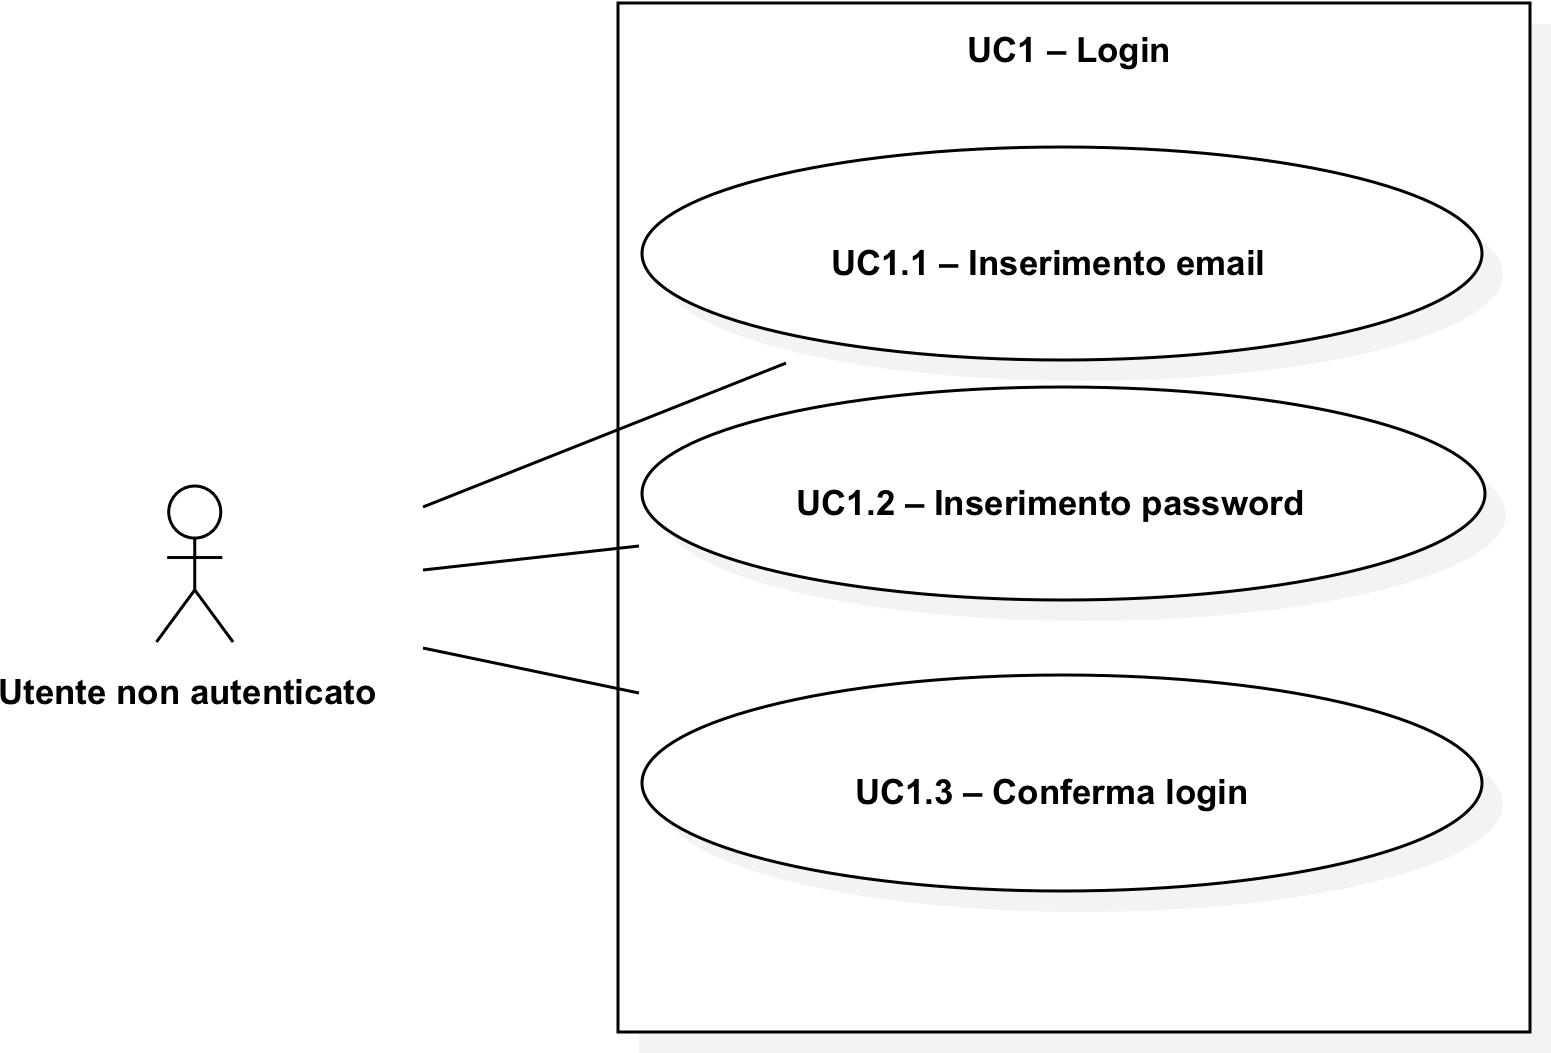
\includegraphics[scale=0.2]{img/UC1.png} 
\caption{Caso d'uso UC1 - Login} 
 \end{figure} 
\desc{l'utente effettua il login con le proprie credenziali.}\\\\ 
\pre{l'utente è registrato presso il database.}\\\\ 
\post{l'utente è autenticato.}\\\\ 
\scen{\begin{itemize}
\item \UC{UC1.1} l'utente inserisce l'email;
\item \UC{UC1.2} l'utente inserisce la password;
\item \UC{UC1.3} l'utente conferma di voler eseguire il login.
\end{itemize}}\\\\ 
\scensec{\begin{itemize}
\item ESTENSIONE: se i dati inseriti non sono corretti l'esecuzione prosegue con \UC{UC14};
\item ESTENSIONE: se l'utente non ricorda le proprie credenziali di accesso può recuperarle grazie a \UC{UC20}.
\end{itemize}}\\\\ 
\att{Utente non autenticato.}

\casoduso{UC1.1}{Inserimento email} 
\desc{l'utente inserisce l'indirizzo email con cui si è registrato in precedenza.}\\\\ 
\pre{la connessione ad internet è attiva e l'app fornisce la pagina di login.}\\\\ 
\post{l'utente ha inserito la mail.}\\\\ 
\scen{l'utente inserisce l'indirizzo email con cui si è registrato in precedenza.}\\\\ 
\att{Utente non autenticato.}

\casoduso{UC1.2}{Inserimento password} 
\desc{l'utente inserisce la password con cui si è registrato in precedenza rispettando il requisito \Req{R0F1.2.6.4}.}\\\\ 
\pre{la connessione ad internet è attiva e l'app fornisce la pagina di login.}\\\\ 
\post{l'utente ha inserito la password.}\\\\ 
\scen{l'utente inserisce la password con cui si è registrato in precedenza rispettando il requisito \Req{R0F1.2.6.4}.}\\\\ 
\att{Utente non autenticato.}

\casoduso{UC1.3}{Conferma Login} 
\desc{l'utente conferma di voler procedere con l'autenticazione con i dati precedentemente inseriti.}\\\\ 
\pre{la connessione ad internet è attiva e l'app fornisce la pagina di login.}\\\\ 
\post{l'utente è stato autenticato.}\\\\ 
\scen{l'utente conferma di voler procedere con l'autenticazione con i dati precedentemente inseriti.}\\\\ 
\att{Utente non autenticato.}

\casoduso{UC10}{Visualizza edificio} 
\begin{figure}[H] 
\centering 
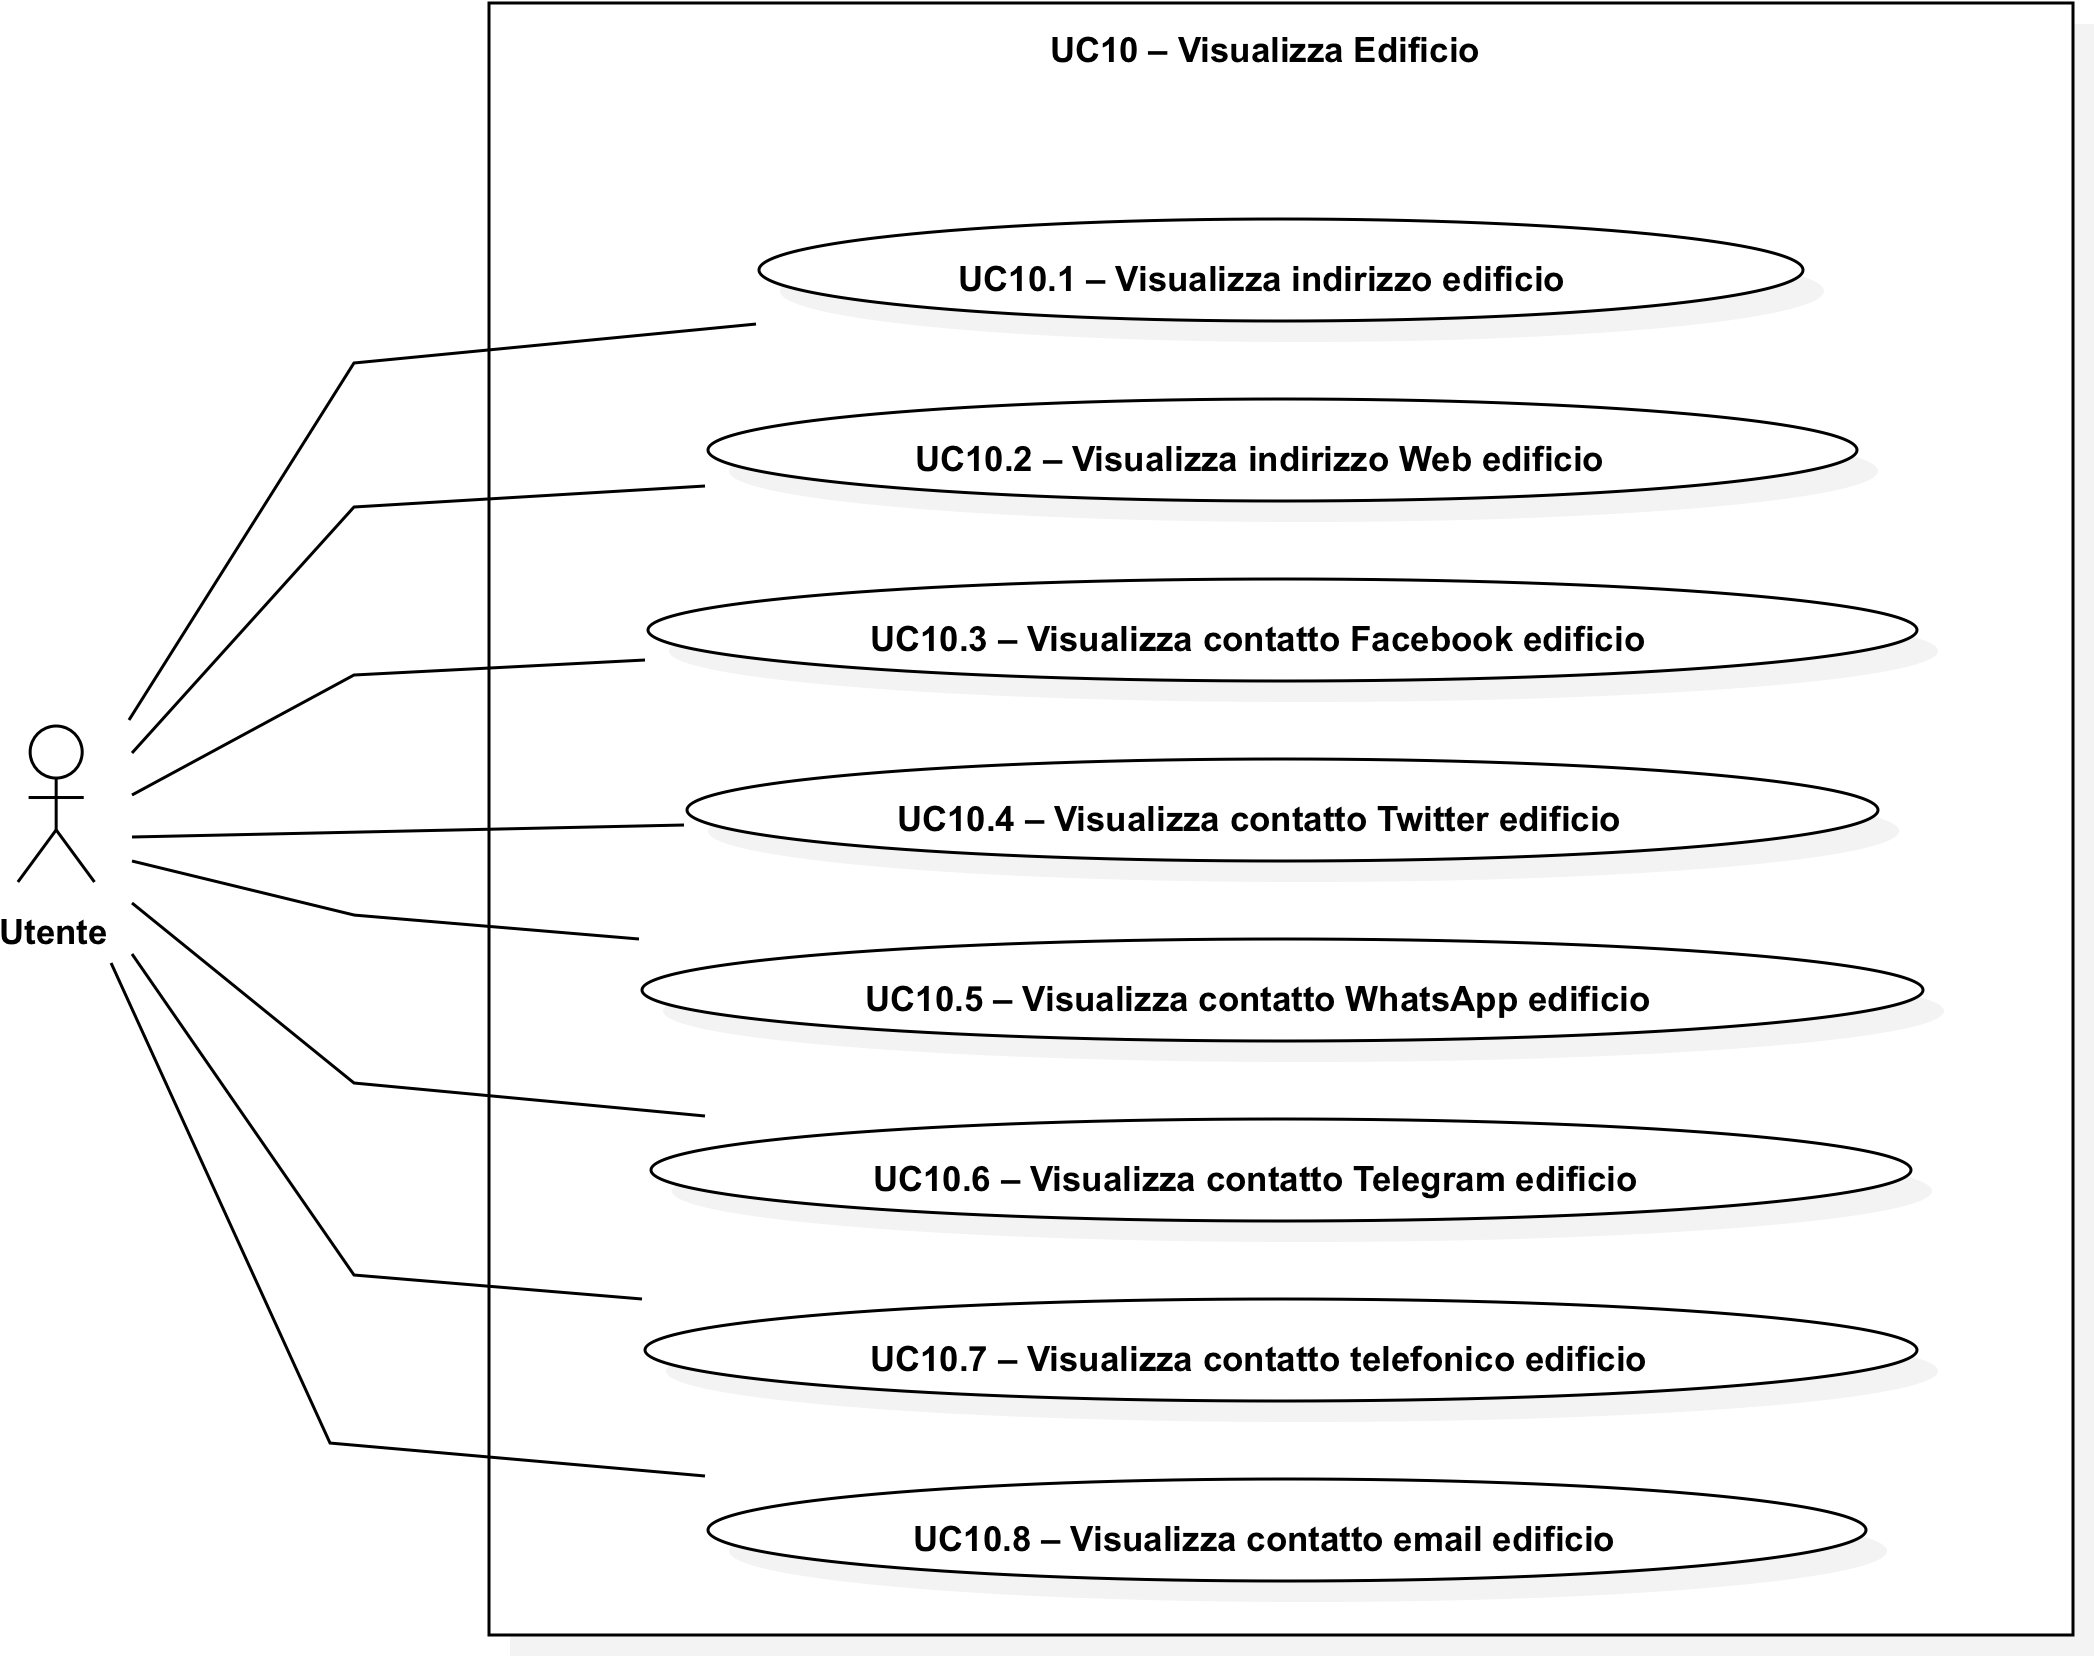
\includegraphics[scale=0.2]{img/UC10.png} 
\caption{Caso d'uso UC10 - Visualizza edificio} 
 \end{figure} 
\desc{l'utente visualizza i dettagli di un edificio abilitato.}\\\\ 
\pre{l'utente ha visualizzato la lista degli edifici abilitati.}\\\\ 
\post{l'utente ha visualizzato i dettagli di un edificio abilitato.}\\\\ 
\scen{l'utente visualizza i dettagli di un edificio abilitato. In particolare visualizza:
\begin{itemize}
\item l'indirizzo (\UC{UC10.1});
\item l'indirizzo web dell' edificio (\UC{UC10.2});
\item i seguenti contatti:
\begin{itemize}
\item Facebook (\UC{UC10.3});
\item Twitter (\UC{UC10.4});
\item WhatsApp (\UC{UC10.5});
\item Telegram (\UC{UC10.6});
\item contatto telefonico (\UC{UC10.7});
\item email (\UC{UC10.7}).
\end{itemize} 
\end{itemize}}\\\\ 
\att{Utente.}

\casoduso{UC10.1}{Visualizza indirizzo edificio} 
\desc{l'utente visualizza l'indirizzo dell'edificio.}\\\\ 
\pre{l'utente richiede informazioni sull'edificio.}\\\\ 
\post{l'utente ha visualizzato l'indirizzo dell'edificio.}\\\\ 
\scen{l'utente visualizza l'indirizzo dell'edificio.}\\\\ 
\att{Utente.}

\casoduso{UC10.2}{Visualizza indirizzo web edificio} 
\desc{l'utente visualizza l'indirizzo web dell'edificio.}\\\\ 
\pre{l'utente richiede informazioni sull'edificio.}\\\\ 
\post{l'utente ha visualizzato l'indirizzo web dell'edificio.}\\\\ 
\scen{l'utente visualizza l'indirizzo web dell'edificio.}\\\\ 
\att{Utente.}

\casoduso{UC10.3}{Visualizza contatto Facebook edificio} 
\desc{l'utente visualizza il contatto Facebook dell'edificio.}\\\\ 
\pre{l'utente richiede informazioni per contattare l'edificio.}\\\\ 
\post{l'utente ha visualizzato il contatto Facebook dell'edificio.}\\\\ 
\scen{l'utente visualizza il contatto Facebook dell'edificio.}\\\\ 
\att{Utente.}

\casoduso{UC10.4}{Visualizza contatto Twitter edificio} 
\desc{l'utente visualizza il contatto Twitter dell'edificio.}\\\\ 
\pre{l'utente richiede informazioni per contattare l'edificio.}\\\\ 
\post{l'utente ha visualizzato il contatto Twitter dell'edificio.}\\\\ 
\scen{l'utente visualizza il contatto Twitter dell'edificio.}\\\\ 
\att{Utente.}

\casoduso{UC10.5}{Visualizza contatto WhatsApp edificio} 
\desc{l'utente visualizza il contatto WhatsApp dell'edificio.}\\\\ 
\pre{l'utente richiede informazioni per contattare l'edificio.}\\\\ 
\post{l'utente ha visualizzato il contatto WhatsApp dell'edificio.}\\\\ 
\scen{l'utente visualizza il contatto WhatsApp dell'edificio.}\\\\ 
\att{Utente.}

\casoduso{UC10.6}{Visualizza contatto Telegram edificio} 
\desc{l'utente visualizza il contatto Telegram dell'edificio.}\\\\ 
\pre{l'utente richiede informazioni per contattare l'edificio.}\\\\ 
\post{l'utente ha visualizzato il contatto Telegram dell'edificio.}\\\\ 
\scen{l'utente visualizza il contatto Telegram dell'edificio.}\\\\ 
\att{Utente.}

\casoduso{UC10.7}{Visualizza contatto telefonico ufficio} 
\desc{l'utente visualizza il contatto telefonico dell'edificio.}\\\\ 
\pre{l'utente richiede informazioni per contattare l'edificio.}\\\\ 
\post{l'utente ha visualizzato il contatto telefonico dell'edificio.}\\\\ 
\scen{l'utente visualizza il contatto telefonico dell'edificio.}\\\\ 
\att{Utente.}

\casoduso{UC10.8}{Visualizza email edificio} 
\desc{l'utente visualizza l'email per contattare  l'edificio.}\\\\ 
\pre{l'utente richiede informazioni per contattare l'edificio.}\\\\ 
\post{l'utente ha visualizzato l'email per contattare  l'edificio.}\\\\ 
\scen{l'utente visualizza l'email per contattare  l'edificio.}\\\\ 
\att{Utente.}

\casoduso{UC11}{Registrazione} 
\begin{figure}[H] 
\centering 
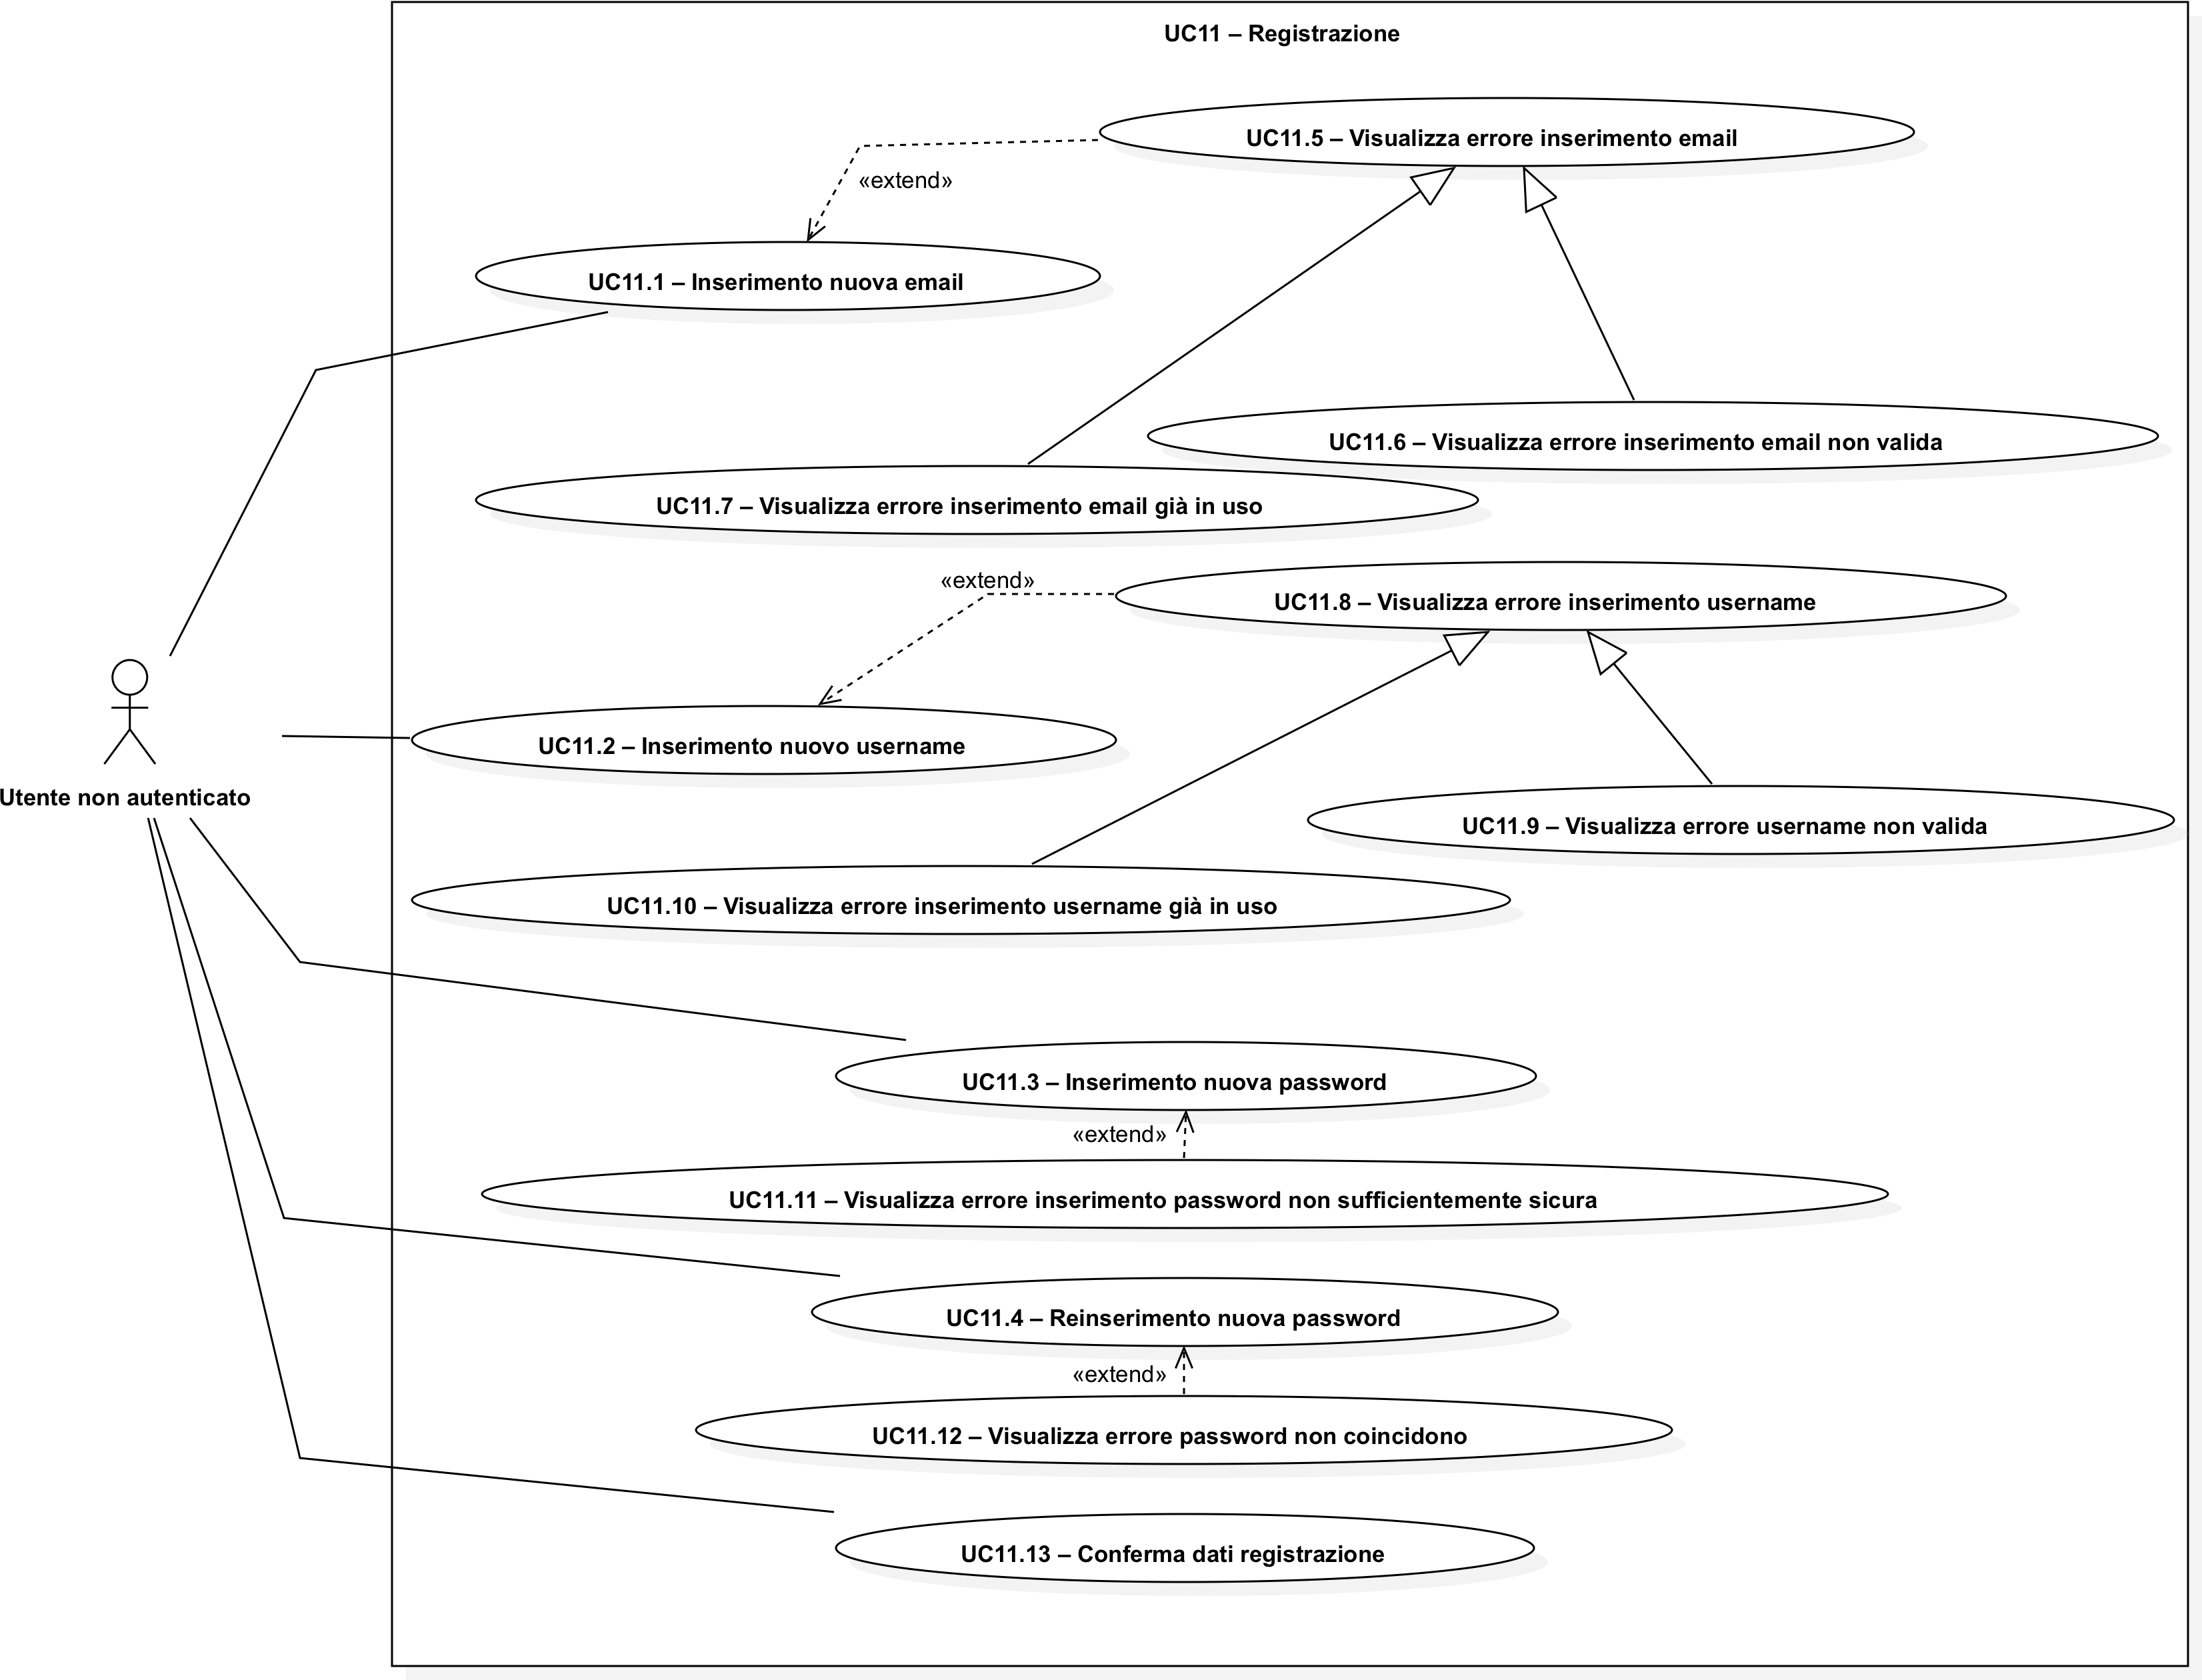
\includegraphics[scale=0.14]{img/UC11.png} 
\caption{Caso d'uso UC11 - Registrazione} 
 \end{figure} 
\desc{l'utente si registra nel database inserendo un'email valida e una password sufficientemente sicura.}\\\\ 
\pre{l'utente non è registrato.}\\\\ 
\post{l'utente è registrato nel database.}\\\\ 
\scen{\begin{itemize}
\item \UC{UC11.1} l'utente inserisce un indirizzo email valido;
\item \UC{UC11.2} l'utente inserisce un username univoco;
\item \UC{UC11.3} l'utente inserisce una password sufficientemente sicura;
\item \UC{UC11.4} l'utente reinserisce la password precedentemente scelta;
\item \UC{UC11.13} l'utente conferma i dati inseriti.
\end{itemize}}\\\\ 
\att{Utente non autenticato.}

\casoduso{UC11.1}{Inserimento nuova email} 
\desc{l'utente inserisce l'indirizzo email con cui desidera registrarsi.}\\\\ 
\pre{la connessione ad internet è attiva e l'App fornisce la pagina di registrazione.}\\\\ 
\post{l'utente ha inserito la email.}\\\\ 
\scen{l'utente inserisce il proprio indirizzo email per registrarsi.}\\\\ 
\scensec{ESTENSIONE \begin{itemize}
\item \UC{UC11.5} l'email inserita non è valida e viene visualizzato l'errore.
\end{itemize}}\\\\ 
\att{Utente non autenticato.}

\casoduso{UC11.10}{Visualizza errore inserimento username già in uso} 
\desc{l'utente viene informato di aver inserito un username già in uso nel sistema.}\\\\ 
\pre{l'utente ha inserito un username già in uso nel sistema.}\\\\ 
\post{l'utente è stato informato di aver inserito un username già in uso nel sistema.}\\\\ 
\scen{l'utente viene informato di aver inserito un username già in uso nel sistema.}\\\\ 
\att{Utente non autenticato.}

\casoduso{UC11.11}{Visualizza errore password non sufficientemente sicura} 
\desc{l'utente visualizza l'errore il quale segnala che la nuova password inserita non è sufficientemente sicura.}\\\\ 
\pre{l'utente ha inserito una nuova password non sufficientemente sicura.}\\\\ 
\post{l'utente ha visualizzato l'errore il quale segnala che la nuova password inserita non è sufficientemente sicura.}\\\\ 
\scen{l'utente visualizza l'errore il quale segnala che la nuova password inserita non è sufficientemente sicura.}\\\\ 
\att{Utente non autenticato.}

\casoduso{UC11.12}{Visualizza errore password reinserita non coincidente con la nuova password} 
\desc{l'utente visualizza l'errore il quale segnala che la password reinserita non coincide con la nuova password.}\\\\ 
\pre{l'utente ha reinserito la password che non coincide con quella nuova precedentemente inserita.}\\\\ 
\post{l'utente ha visualizzato l'errore il quale segnala che la password reinserita non coincide con la nuova password.}\\\\ 
\scen{l'utente visualizza l'errore il quale segnala che la password reinserita non coincide con la nuova password.}\\\\ 
\att{Utente non autenticato.}

\casoduso{UC11.13}{Conferma dati registrazione} 
\desc{l'utente conferma i dati di registrazione inseriti.}\\\\ 
\pre{l'utente ha inserito i dati per la registrazione.}\\\\ 
\post{l'utente ha confermato i dati inseriti per la registrazione.}\\\\ 
\scen{l'utente conferma i dati di registrazione inseriti.}\\\\ 
\att{Utente non autenticato.}

\casoduso{UC11.2}{Inserimento nuovo username} 
\desc{l'utente inserisce l'username con cui desidera registrarsi.}\\\\ 
\pre{la connessione ad internet è attiva e l'App fornisce la pagina di registrazione.}\\\\ 
\post{l'utente ha inserito l'username.}\\\\ 
\scen{l'utente inserisce l'username con cui desidera registrarsi.}\\\\ 
\scensec{ESTENSIONE \begin{itemize}
\item \UC{UC11.6} l'username inserito è già in uso e viene visualizzato l'errore.
\end{itemize}}\\\\ 
\att{Utente non autenticato.}

\casoduso{UC11.3}{Inserimento nuova password} 
\desc{l'utente inserisce la password con cui desidera registrarsi.}\\\\ 
\pre{la connessione ad internet è attiva e l'App fornisce la pagina di registrazione.}\\\\ 
\post{l'utente ha inserito la password.}\\\\ 
\scen{l'utente inserisce la password con cui desidera registrarsi.}\\\\ 
\scensec{ESTENSIONE \begin{itemize}
\item \UC{UC11.11} la password inserita non è sufficientemente sicura e viene visualizzato l'errore.
\end{itemize}}\\\\ 
\att{Utente non autenticato.}

\casoduso{UC11.4}{Reinserimento nuova password} 
\desc{l'utente reinserisce la nuova password.}\\\\ 
\pre{l'utente si trova nella pagina di registrazione.}\\\\ 
\post{l'utente ha reniserito la nuova password.}\\\\ 
\scen{l'utente reinserisce la nuova password.}\\\\ 
\scensec{ESTENSIONE \begin{itemize}
\item \UC{UC11.12}: la password reinserita non coincide con la nuova password e viene visualizzato l'errore.
\end{itemize}}\\\\ 
\att{Utente non autenticato.}

\casoduso{UC11.5}{Visualizza errore inserimento email} 
\desc{l'utente visualizza l'errore il quale segnala che l'email non rispetta i requisiti richiesti.}\\\\ 
\pre{l'utente ha inserito una email non rispetta i requisiti richiesti.}\\\\ 
\post{l'utente ha visualizzato l'errore il quale segnala che l'email non rispetta i requisiti richiesti.}\\\\ 
\scen{l'utente visualizza l'errore il quale segnala che l'email non rispetta i requisiti richiesti}\\\\ 
\att{Utente non autenticato.}

\casoduso{UC11.6}{Visualizza errore inserimento email non valida} 
\desc{l'utente visualizza un messaggio d'errore perché ha inserito un'email  non valida che non soddisfa il \Req{R0F1.2.7.1.1}.}\\\\ 
\pre{l'utente ha inserito un'email non valida.}\\\\ 
\post{l'utente viene notificato di aver inserito un'email non valida.}\\\\ 
\scen{l'utente visualizza un messaggio d'errore perché ha inserito un'email  non valida che non soddisfa il \Req{R0F1.2.7.1.1}.}\\\\ 
\att{Utente non autenticato.}

\casoduso{UC11.7}{Visualizza errore inserimento email già in uso} 
\desc{l'utente viene notificato di aver inserito un'email già presente nel sistema.}\\\\ 
\pre{l'utente ha inserito un'email già presente nel sistema.}\\\\ 
\post{l'utente è stato notificato di aver inserito un'email già presente nel sistema.}\\\\ 
\scen{l'utente viene notificato di aver inserito un'email già presente nel sistema.}\\\\ 
\att{Utente non autenticato.}

\casoduso{UC11.8}{Visualizza errore inserimento username} 
\desc{l'utente visualizza l'errore sull'inserimento dell'username.}\\\\ 
\pre{l'utente ha inserito un nuovo username che non soddisfa i requisiti richiesti.}\\\\ 
\post{l'utente ha visualizzato il messaggio di errore sull'inserimento dell'username.}\\\\ 
\scen{l'utente visualizza l'errore sull'inserimento dell'username.}\\\\ 
\att{Utente non autenticato.}

\casoduso{UC11.9}{Visualizza errore inserimento username non valido} 
\desc{l'utente ha inserito un username che non rispetta il requisito \Req{R0F1.2.7.2.1}.}\\\\ 
\pre{l'utente ha inserito un username non valido.}\\\\ 
\post{l'utente viene notificato di aver inserito un username non valido.}\\\\ 
\scen{l'utente ha inserito un username che non rispetta il requisito \Req{R0F1.2.7.2.1}.}\\\\ 
\att{Utente non autenticato.}

\casoduso{UC12}{Visualizza avviso di attivazione GPS} 
\desc{l'utente visualizza il messaggio di invito all'attivazione del GPS.}\\\\ 
\pre{il GPS non è attivo sul dispositivo dell'utente.}\\\\ 
\post{l'utente ha visualizzato il messaggio di invito all'attivazione del GPS.}\\\\ 
\scen{l'utente visualizza il messaggio di invito all'attivazione del GPS.}\\\\ 
\att{Utente.}

\casoduso{UC13}{Visualizza avviso di attivazione della connessione ad internet} 
\desc{l'utente visualizza il messaggio di invito all'attivazione della connessione ad internet.}\\\\ 
\pre{la connessione ad internet non è attiva sul dispositivo dell'utente.}\\\\ 
\post{l'utente ha visualizzato il messaggio di invito all'attivazione della connessione ad internet.}\\\\ 
\scen{l'utente visualizza il messaggio di invito all'attivazione della connessione ad internet.}\\\\ 
\att{Utente.}

\casoduso{UC14}{Errore autenticazione} 
\desc{L'utente visualizza l'errore di autenticazione nel quale viene specificato che non ha inserito i dati corretti.}\\\\ 
\pre{l'utente ha inserito i dati di autenticazione.}\\\\ 
\post{l'utente ha visualizzato l'errore di autenticazione.}\\\\ 
\scen{L'utente visualizza l'errore di autenticazione nel quale viene specificato che non ha inserito i dati corretti.}\\\\ 
\att{Utente non autenticato.}

\casoduso{UC15}{Visualizza lista percorsi salvati} 
\desc{l'utente visualizza la lista dei percorsi salvati.}\\\\ 
\pre{l'utente ha l'app installata e in esecuzione.}\\\\ 
\post{l'utente ha visualizzato i percorsi salvati.}\\\\ 
\scen{l'utente visualizza la lista dei percorsi salvati.}\\\\ 
\scensec{ESTENSIONE: \begin{itemize}
\item \UC{UC17} l'utente non è autenticato e visualizza l'invito ad autenticarsi per visualizzare la lista dei percorsi salvati;
\item \UC{UC18} l'utente visualizza l'invito a registrarsi per poi autenticarsi e visualizzare la lista dei percorsi salvati;
\item \UC{UC19} l'utente non ha alcun percorso salvato e visualizza l'invito a svolgerene almeno uno.
\end{itemize}}\\\\ 
\att{Utente.}

\casoduso{UC16}{Visualizza invito ad autenticarsi} 
\desc{l'utente visualizza l'invito ad autenticarsi.}\\\\ 
\pre{l'utente non è autenticato.}\\\\ 
\post{l'utente ha visualizzato l'invito ad autenticarsi.}\\\\ 
\scen{l'utente visualizza l'invito ad autenticarsi.}\\\\ 
\att{Utente non autenticato.}

\casoduso{UC17}{Visualizza invito a registrarsi} 
\desc{l'utente visualizza l'invito a registrarsi.}\\\\ 
\pre{l'utente non è registrato nel database dell'app.}\\\\ 
\post{l'utente ha visualizzato l'invito a registrarsi.}\\\\ 
\scen{l'utente visualizza l'invito a registrarsi.}\\\\ 
\att{Utente non autenticato.}

\casoduso{UC18}{Visualizza invito a svolgere un percorso} 
\desc{l'utente visualizza l'invito a svolgere almeno un percorso.}\\\\ 
\pre{l'utente non ha svolto nessun percorso.}\\\\ 
\post{l'utente ha visualizzato l'invito a svolgere almeno un percorso.}\\\\ 
\scen{l'utente visualizza l'invito a svolgere almeno un percorso.}\\\\ 
\att{Utente.}

\casoduso{UC19}{Visualizza dettagli percorso salvato} 
\desc{l'utente visualizza i dettagli di un percorso salvato.}\\\\ 
\pre{l'utente ha salvato almeno un percorso.}\\\\ 
\post{l'utente ha visualizzato i dettagli di un percorso salvato.}\\\\ 
\scen{l'utente visualizza i dettagli di un percorso salvato.}\\\\ 
\att{Utente autenticato.}

\casoduso{UC2}{Deautenticazione} 
\desc{l'utente autenticato esegue il logout.}\\\\ 
\pre{l'utente è autenticato.}\\\\ 
\post{l'utente non è più autenticato.}\\\\ 
\scen{l'utente autenticato esegue il logout.}\\\\ 
\att{Utente autenticato.}

\casoduso{UC20}{Recupero credenziali} 
\begin{figure}[H] 
\centering 
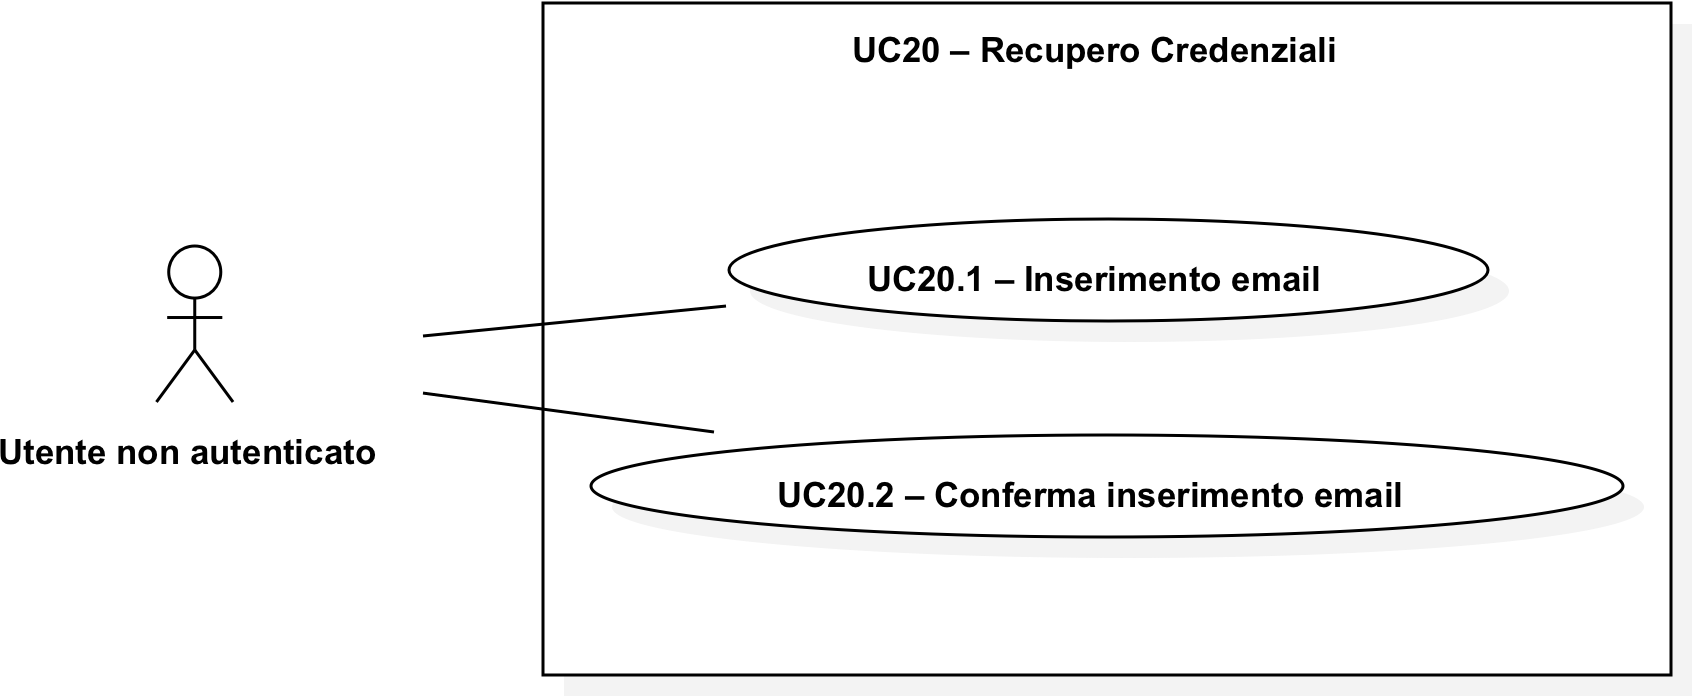
\includegraphics[scale=0.2]{img/UC20.png} 
\caption{Caso d'uso UC20 - Recupero credenziali} 
 \end{figure} 
\desc{l'utente richiede le credenziali d'accesso.}\\\\ 
\pre{l'utente non ricorda le credenziali per accedere al suo profilo.}\\\\ 
\post{l'utente ha richiesto le proprie credenziali di acesso.}\\\\ 
\scen{l'utente richiede le credenziali d'accesso:
\begin{itemize}
\item \UC{UC20.1} l'utente inserisce l'email con cui è registrato
\item \UC{UC20.2} l'utente conferma l'email inserita.
\end{itemize}}\\\\ 
\att{Utente non autenticato.}

\casoduso{UC20.1}{Inserimento email} 
\desc{l'utente inserisce l'email con cui si era registrato.}\\\\ 
\pre{l'utente non riesce ad effettuare il login perché non è in possesso delle credenziali.}\\\\ 
\post{l'utente ha inserito l'email con cui si era registrato.}\\\\ 
\scen{l'utente inserisce l'email con cui si era registrato.}\\\\ 
\att{Utente non autenticato.}

\casoduso{UC20.2}{Conferma inserimento email} 
\desc{l'utente conferma l'email che ha inserito per il recupero delle credenziali.}\\\\ 
\pre{l'utente ha inserito l'email per il recupero delle credenziali.}\\\\ 
\post{l'utente ha confermato l'inserimento della mail per il recupero delle credenziali.}\\\\ 
\scen{l'utente conferma l'email che ha inserito per il recupero delle credenziali.}\\\\ 
\att{Utente non autenticato.}

\casoduso{UC21}{Visualizza percorsi disponibili} 
\desc{l'utente visualizza i percorsi disponibili nell'edificio in cui si trova.}\\\\ 
\pre{l'utente ha attivato i servizi di localizzazione, bluetooth e la connessione ad Internet; l'utente è in un edificio abilitato; l'utente è in prossimità di un beacon.}\\\\ 
\post{l'utente ha visualizzato la lista dei percorsi disponibili.}\\\\ 
\scen{l'utente visualizza i percorsi disponibili nell'edificio in cui si trova}\\\\ 
\att{Utente.}

\casoduso{UC22}{Visualizza lista dei percorsi percorsi} 
\desc{l'utente visualizza la lista dei percorsi presenti nell'edificio.}\\\\ 
\pre{l'utente ha i servizi di localizzazione, bluetooth e connessione a Internet attivi.}\\\\ 
\post{l'utente ha visualizzato i percorsi presenti nell'edificio.}\\\\ 
\scen{l'utente visualizza la lista dei percorsi presenti nell'edificio}\\\\ 
\att{Utente.}

\casoduso{UC23}{Visualizza percorso} 
\desc{l'utente visualizza i dettagli di un percorso.}\\\\ 
\pre{l'utente ha visualizzato la lista degli edifici.}\\\\ 
\post{l'utente ha visualizzato i dettagli di un percorso.}\\\\ 
\scen{l'utente visualizza i dettagli di un percorso e se si trova nell'edificio del percorso può:
\begin{itemize}
\item UC{UC3} iniziare a svolgere il percorso.
\end{itemize}}\\\\ 
\att{Utente.}

\casoduso{UC3}{Svolgimento del percorso} 
\begin{figure}[H] 
\centering 
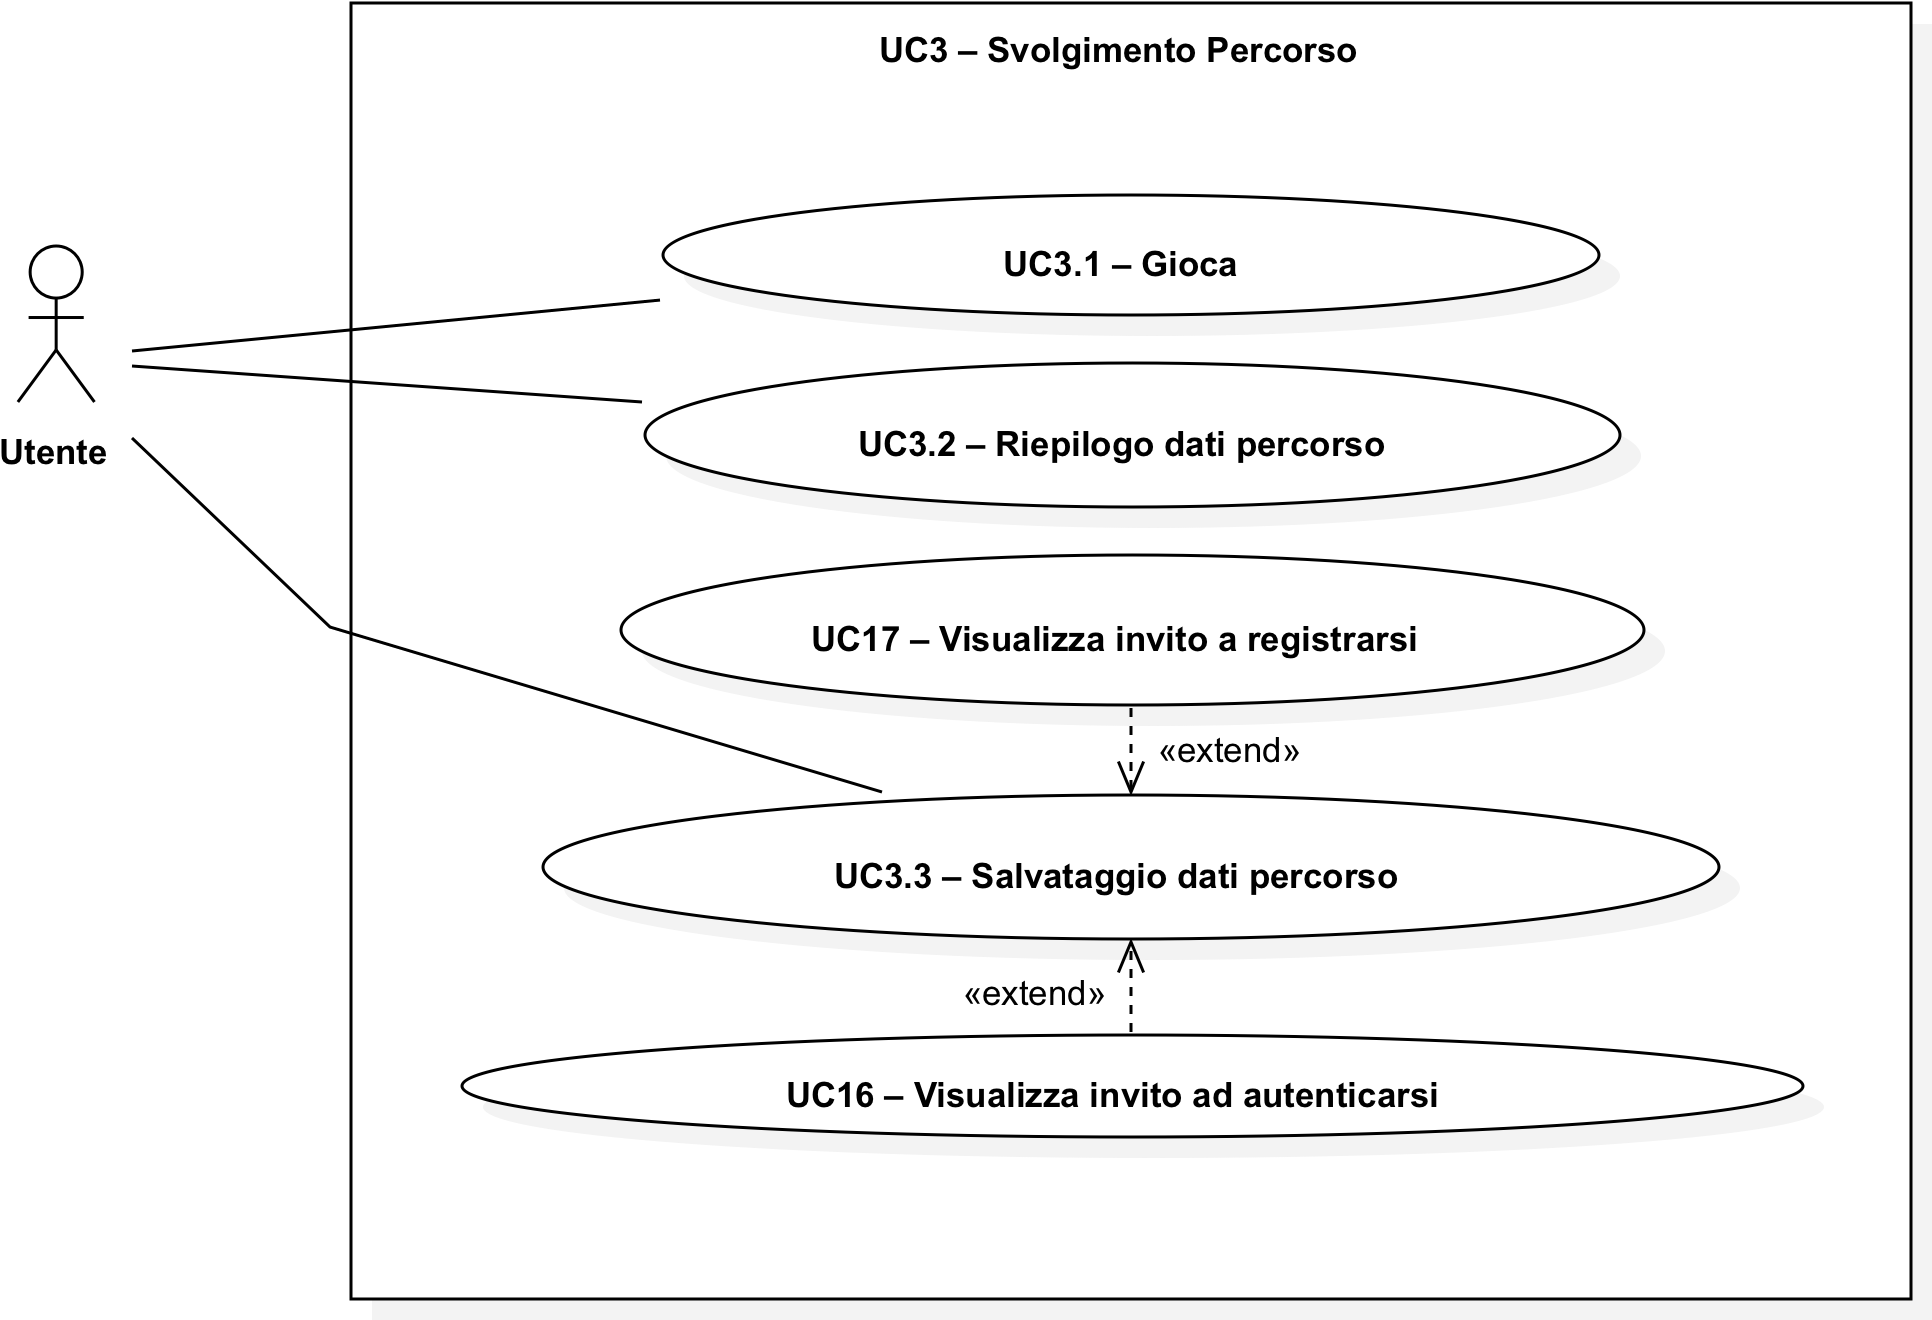
\includegraphics[scale=0.2]{img/UC3.png} 
\caption{Caso d'uso UC3 - Svolgimento del percorso} 
 \end{figure} 
\desc{l'utente svolge un percorso tra quelli disponibili nel luogo in cui si trova.}\\\\ 
\pre{l'utente ha i servizi di localizzazione, il Bluetooth e la connessione ad internet attivi e si trova in un luogo abilitato.}\\\\ 
\post{l'utente ha completato il percorso selezionato.}\\\\ 
\scen{l'utente effettua i seguenti passi:
\begin{itemize}
\item \UC{UC3.1} l'utente gioca il percorso;
\item \UC{UC3.2} l'utente visualizza i dati del percorso appena concluso;
\item \UC{UC3.3} l'utente autenticato salva i risultati.
\end{itemize}}\\\\ 
\att{Utente.}

\casoduso{UC3.1}{Gioca} 
\begin{figure}[H] 
\centering 
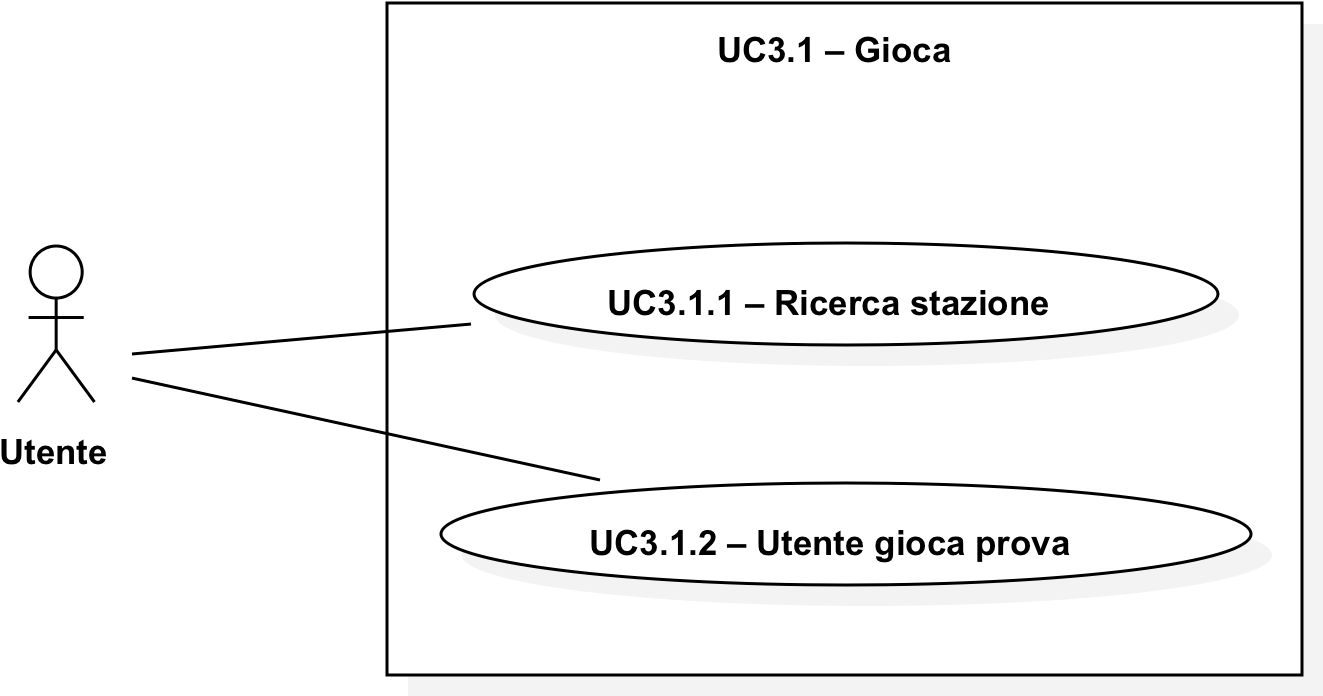
\includegraphics[scale=0.2]{img/UC3_1.png} 
\caption{Caso d'uso UC3.1 - Gioca} 
 \end{figure} 
\desc{l'utente si trova in un luogo abilitato, scarica un percorso e lo conclude.}\\\\ 
\pre{l'utente ha scelto un percorso.}\\\\ 
\post{l'utente completa tutte le prove.}\\\\ 
\scen{\begin{itemize}
\item \UC{UC3.1.1} l'utente ricerca una stazione;
\item \UC{UC3.1.2} l'utente svolge la prova della stazione in cui si trova.
\end{itemize}}\\\\ 
\att{Utente.}

\casoduso{UC3.1.1}{Ricerca stazione} 
\desc{l'utente è alla ricerca della stazione in cui recarsi per la prossima o la prima prova.}\\\\ 
\pre{l'utente non sta svolgendo alcuna prova e non ha concluso il percorso.}\\\\ 
\post{l'utente è presso la stazione in cui svolgere la prossima prova.}\\\\ 
\scen{l'utente è alla ricerca della stazione in cui recarsi per la prossima o la prima prova.}\\\\ 
\att{Utente.}

\casoduso{UC3.1.2}{Utente gioca prova} 
\begin{figure}[H] 
\centering 
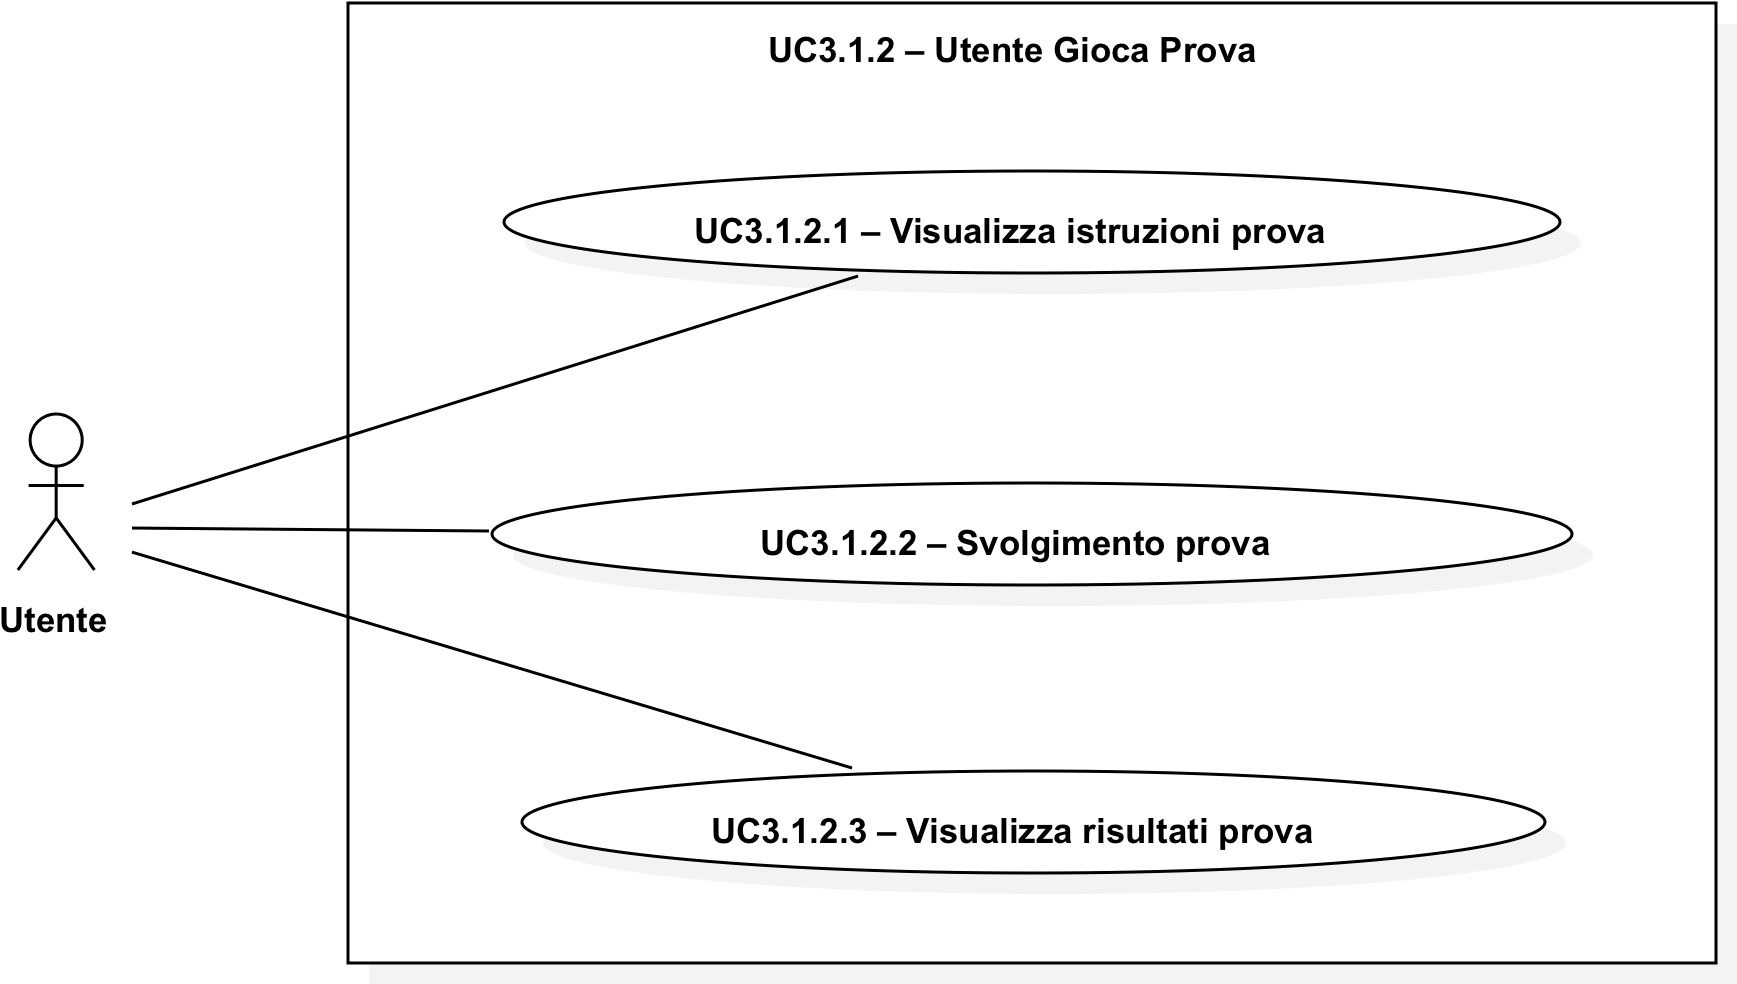
\includegraphics[scale=0.2]{img/UC3_1_2.png} 
\caption{Caso d'uso UC3.1.2 - Utente gioca prova} 
 \end{figure} 
\desc{l'utente affronta la prova della stazione in cui si trova.}\\\\ 
\pre{l'utente si trova nella sua prossima stazione.}\\\\ 
\post{l'utente ha completato la prova.}\\\\ 
\scen{\begin{itemize}
\item \UC{UC3.1.2.1} l'utente visualizza una descrizione della prova;
\item \UC{UC3.1.2.2} l'utente gioca la prova;
\item \UC{UC3.1.2.3} l'utente ottiene un punteggio sulla prova.
\end{itemize}}\\\\ 
\att{Utente.}

\casoduso{UC3.1.2.1}{Visualizza istruzioni prova} 
\desc{l'utente visualizza le informazioni che deve sapere in preparazione alla prova, solitamente le istruzioni (il tempo per la prova non scorre ancora).}\\\\ 
\pre{l'utente è in procinto di iniziare la prova.}\\\\ 
\post{l'utente ha ricevuto informazioni su come procedere per la prova.}\\\\ 
\scen{l'utente visualizza le informazioni che deve sapere in preparazione alla prova, solitamente le istruzioni (il tempo per la prova non scorre ancora).}\\\\ 
\att{Utente.}

\casoduso{UC3.1.2.2}{Svolgimento prova} 
\desc{l'utente svolge la prova prevista per la stazione.}\\\\ 
\pre{l'utente ha visualizzato le informazioni necessarie allo svolgimento della prova.}\\\\ 
\post{l'utente ha concluso la prova con successo.}\\\\ 
\scen{l'utente svolge la prova prevista per la stazione.}\\\\ 
\att{Utente.}

\casoduso{UC3.1.2.3}{Visualizza risultati prova} 
\desc{l'utente viene informato circa i risultati ottenuti durante la prova appena conclusa.}\\\\ 
\pre{l'utente ha appena concluso una prova.}\\\\ 
\post{l'utente ha ottenuto i risultati circa la prova appena conclusa.}\\\\ 
\scen{l'utente viene informato circa i risultati ottenuti durante la prova appena conclusa.}\\\\ 
\att{Utente.}

\casoduso{UC3.2}{Riepilogo dati 
percorso} 
\begin{figure}[H] 
\centering 
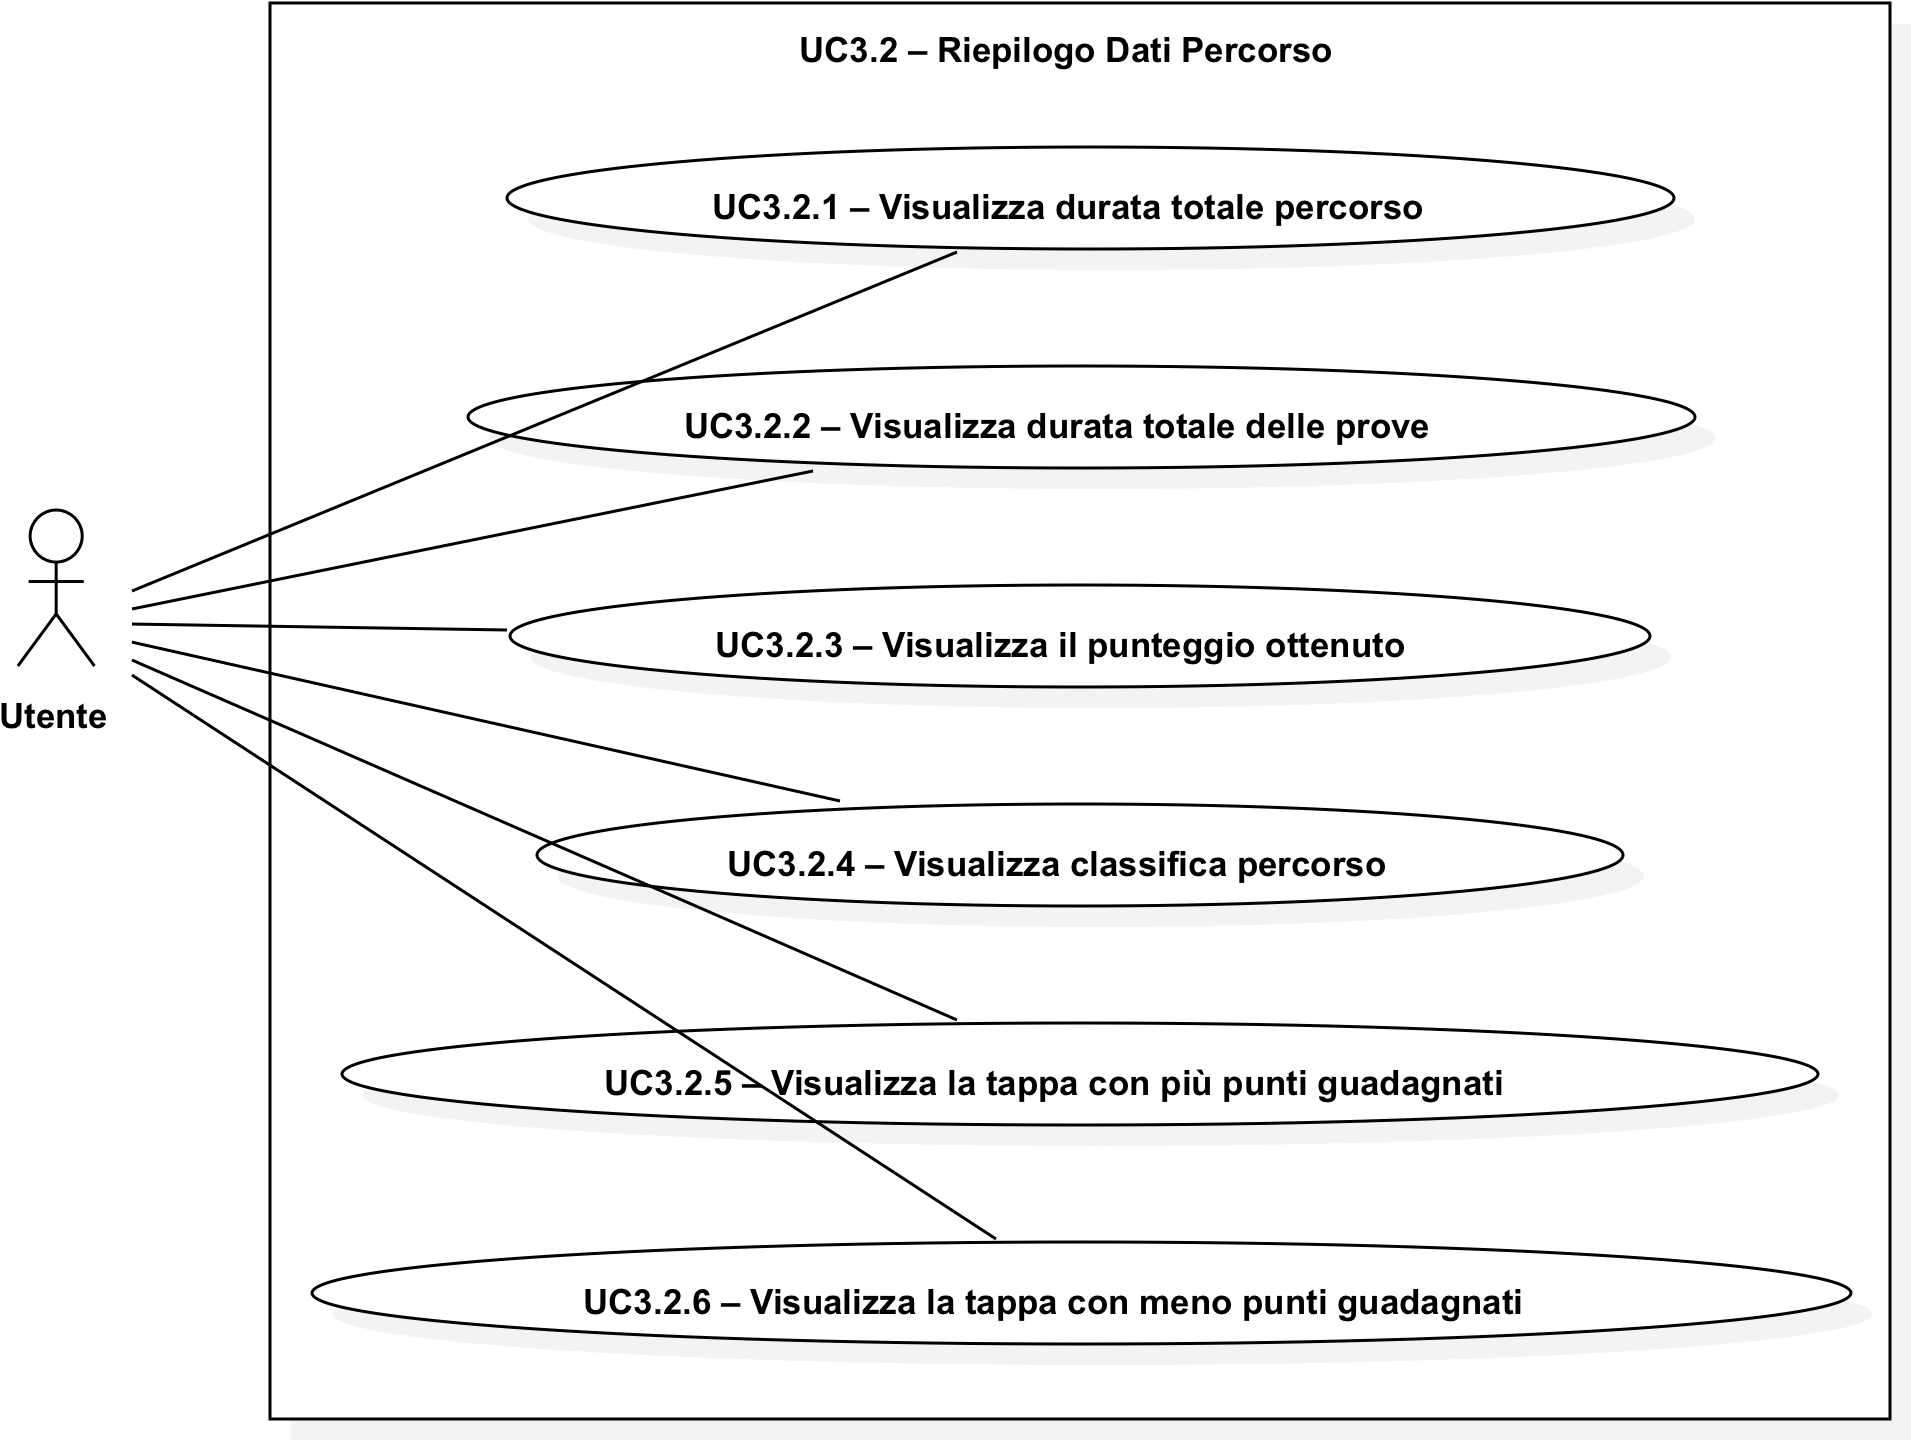
\includegraphics[scale=0.2]{img/UC3_2.png} 
\caption{Caso d'uso UC3.2 - Riepilogo dati percorso} 
 \end{figure} 
\desc{dopo che l'utente termina il percorso visualizza il riassunto: durata totale, durata totale delle prove, punteggio ottenuto, posizione in classifica.}\\\\ 
\pre{l'utente ha completato il percorso.}\\\\ 
\post{l'utente ha visualizzato il riassunto del percorso.}\\\\ 
\scen{L'utente visualizza le seguenti informazioni:
\begin{itemize}
 \item \UC{UC3.2.1} informazioni generali sulla durata (orario di inizio/fine, durata totale);
\item \UC{UC3.2.2} durata delle prove (somma della durata di ciascuna prova);
\item \UC{UC3.2.3} punteggio ottenuto (somma dei punteggi ottenuti nelle varie prove);
\item \UC{UC3.2.4} punteggio medio ottenuto dagli utenti (media dei punteggi ottenuti su quel percorso);
\item \UC{UC3.2.5} visualizza la tappa in cui è stato ottenuto il maggior numero di punti;
\item \UC{UC3.2.6} visualizza la tappa in cui è stato ottenuto il minor numero di punti.
\end{itemize}}\\\\ 
\att{Utente.}

\casoduso{UC3.2.1}{Visualizza durata totale percorso} 
\desc{l'utente visualizza il tempo totale impiegato per il percorso, ovvero il tempo intercorso tra l'orario di inizio e quello di fine.}\\\\ 
\pre{l'utente ha concluso il percorso.}\\\\ 
\post{l'app mostra i dettagli sul tempo di inizio, fine e durata.}\\\\ 
\scen{l'utente visualizza il tempo totale impiegato per il percorso, ovvero il tempo intercorso tra l'orario di inizio e quello di fine}\\\\ 
\att{Utente.}

\casoduso{UC3.2.2}{Visualizza durata totale delle prove} 
\desc{l'utente visualizza la durata totale del percorso: la somma dei tempi spesi dall'utente nel compiere le varie prove.}\\\\ 
\pre{l'utente ha concluso il percorso.}\\\\ 
\post{l'utente ha visualizzato i dettagli sulla durata delle prove.}\\\\ 
\scen{l'utente visualizza la durata totale del percorso: la somma dei tempi spesi dall'utente nel compiere le varie prove.}\\\\ 
\att{Utente.}

\casoduso{UC3.2.3}{Visualizza il punteggio ottenuto} 
\desc{l'utente visualizza il punteggio ottenuto durante il percorso che è composto dalla somma dei punteggi ottenuti nelle varie prove.}\\\\ 
\pre{l'utente ha concluso il percorso.}\\\\ 
\post{l'utente ha visualizzato il punteggio ottenuto.}\\\\ 
\scen{l'utente visualizza il punteggio ottenuto durante il percorso che è composto dalla somma dei punteggi ottenuti nelle varie prove.}\\\\ 
\att{Utente.}

\casoduso{UC3.2.4}{Visualizza classifica del percorso} 
\desc{l'utente visualizza alcune informazioni circa le prime posizioni in classifica, quelle antecedenti e quelle seguenti l'utente nel percorso appena concluso (si veda \Req{R0F3.2.4} e figli).}\\\\ 
\pre{l'utente ha concluso il percorso.}\\\\ 
\post{l'utente ha visualizzato la sua posizione in classifica assoluta ottenuta per quel percorso.}\\\\ 
\scen{l'utente visualizza alcune informazioni circa le prime posizioni in classifica, quelle antecedenti e quelle seguenti l'utente nel percorso appena concluso (si veda \Req{R0F3.2.4} e figli).}\\\\ 
\att{Utente.}

\casoduso{UC3.2.5}{Visualizza la tappa con più punti guadagnati} 
\desc{l'utente visualizza la tappa del percorso appena concluso dove ha accumulato il maggior numero di punti.}\\\\ 
\pre{l'utente ha concluso il percorso.}\\\\ 
\post{l'utente ha visualizzato la prova in cui ha accumulato il maggior numero di punti.}\\\\ 
\scen{l'utente visualizza la tappa del percorso appena concluso dove ha accumulato il maggior numero di punti.}\\\\ 
\att{Utente.}

\casoduso{UC3.2.6}{Visualizza la tappa con meno punti guadagnati} 
\desc{l'utente visualizza la tappa del percorso appena concluso in cui l'utente ha accumulato il minor numero di punti.}\\\\ 
\pre{l'utente ha concluso il percorso.}\\\\ 
\post{l'utente ha visualizzato la prova in cui ha accumulato il minor numero di punti.}\\\\ 
\scen{l'utente visualizza la tappa del percorso appena concluso in cui l'utente ha accumulato il minor numero di punti.}\\\\ 
\att{Utente.}

\casoduso{UC3.3}{Salvataggio dati percorso} 
\desc{l'utente autenticato può salvare i dati relativi al percorso appena conclusosi.}\\\\ 
\pre{si è concluso il percorso, l'utente è autenticato.}\\\\ 
\post{i dati del percorso vengono salvati nel database per una futura consultazione.}\\\\ 
\scen{l'utente autenticato può salvare i dati relativi al percorso appena conclusosi.}\\\\ 
\scensec{ESTENSIONE: \begin{itemize}
\item UC{UC16} l'utente non è autenticato e visualizza l'invito ad autenticarsi per salvare i dati del percorso;
\item UC{UC17} l'utente visualizza l'invito a registrarsi per poi autenticarsi e salvare i dati del percorso.
\end{itemize}}\\\\ 
\att{Utente.}

\casoduso{UC4}{Visualizza informazioni e contatti utili} 
\begin{figure}[H] 
\centering 
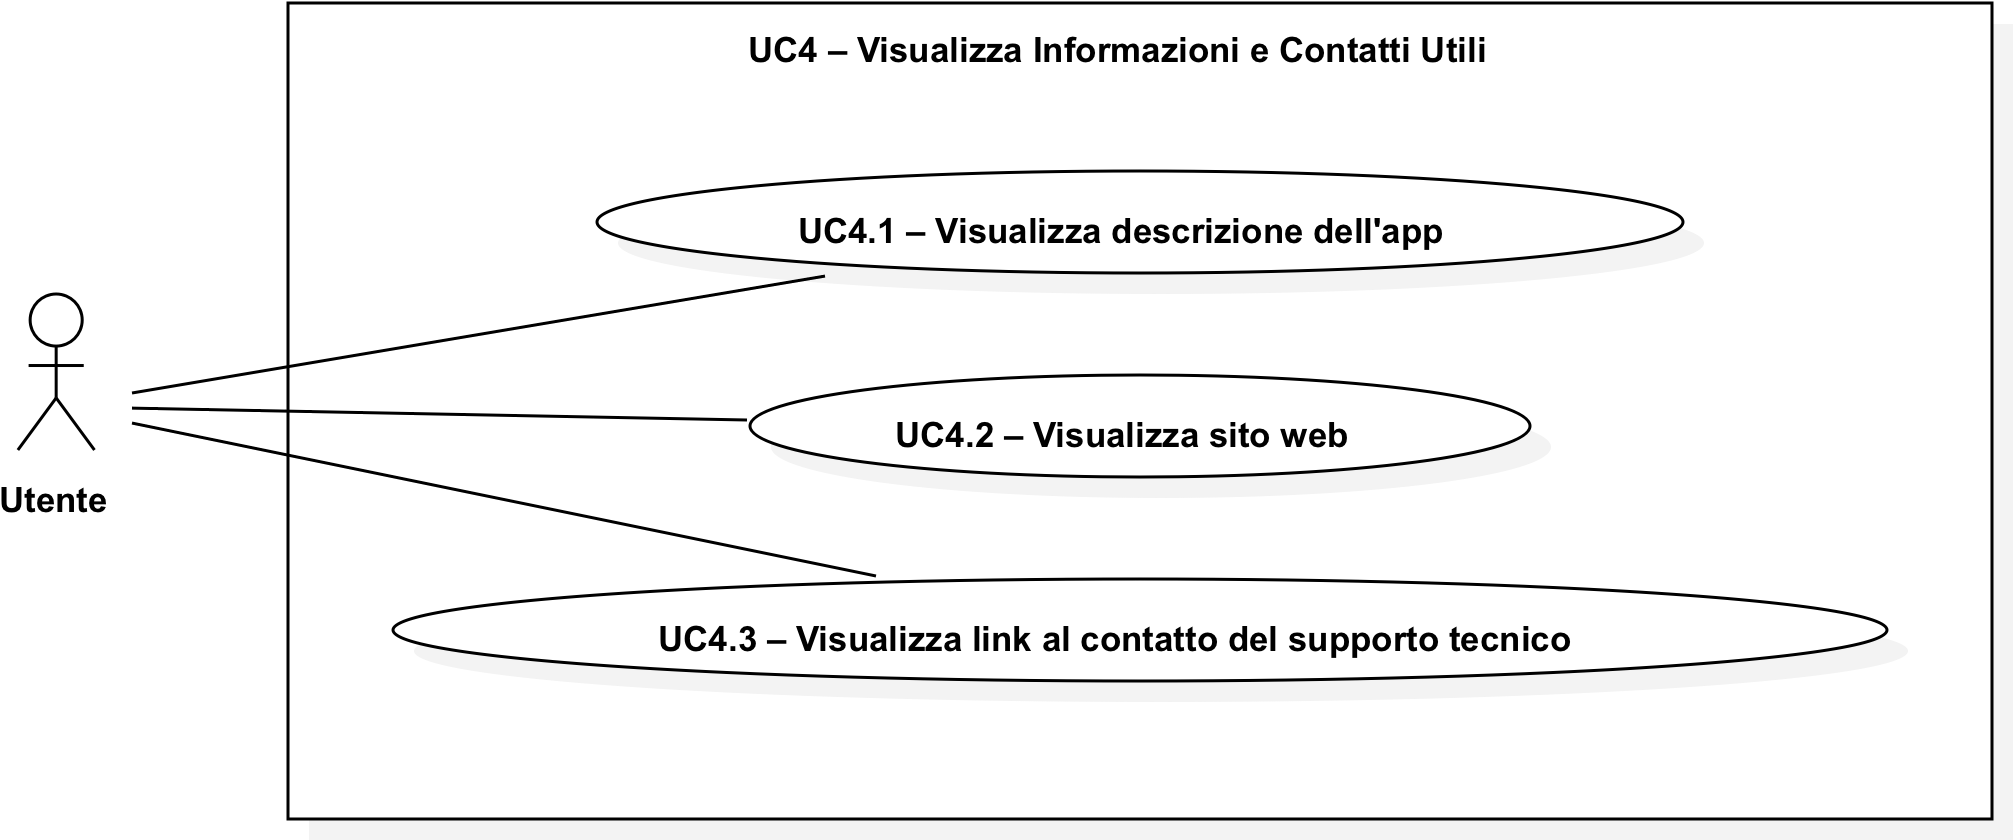
\includegraphics[scale=0.2]{img/UC4.png} 
\caption{Caso d'uso UC4 - Visualizza informazioni e contatti utili} 
 \end{figure} 
\desc{l'utente visualizza le informazioni relative all'app.}\\\\ 
\pre{l'utente ha l'app installata e in esecuzione.}\\\\ 
\post{l'utente si è informato riguardo l'app.}\\\\ 
\scen{\begin{itemize}
\item \UC{UC4.1} l'utente visualizza una descrizione delle funzionalità dell'app;
\item \UC{UC4.2} l'utente visita il sito web dell'app;
\item \UC{UC4.3} l'utente visualizza il contatto al supporto tecnico dell'app.
\end{itemize}}\\\\ 
\att{Utente.}

\casoduso{UC4.1}{Visualizza descrizione dell'app} 
\desc{l'utente visualizza una schermata con un testo esplicativo delle funzionalità dell'app.}\\\\ 
\pre{l'utente ha l'app installata e in esecuzione.}\\\\ 
\post{l'utente ha visualizzato la descrizione delle funzionalità dell'app.}\\\\ 
\scen{l'utente visualizza una schermata con un testo esplicativo delle funzionalità dell'app.}\\\\ 
\att{Utente.}

\casoduso{UC4.2}{Visualizza sito Web} 
\desc{l'utente visualizza il sito web relativo all'app per ottenere maggiori informazioni a riguardo.}\\\\ 
\pre{l'utente è nella pagina di visualizzazione delle informazioni e dei contatti utili.}\\\\ 
\post{l'utente ha visualizzato il sito web relativo all'app tramite il browser del dispositivo.}\\\\ 
\scen{l'utente visualizza il sito web relativo all'app per ottenere maggiori informazioni a riguardo.}\\\\ 
\att{Utente.}

\casoduso{UC4.3}{Visualizza link di contatto al supporto tecnico dell'app} 
\desc{si apre il client email di default nel dispositivo con il campo destinatario impostato all'indirizzo di supporto dell'app per inviare una segnalazione al supporto tecnico.}\\\\ 
\pre{l'utente ha riscontrato un mal funzionamento dell'app.}\\\\ 
\post{l'utente è stato indirizzato al client email di default del dispositivo per inviare una segnalazione al supporto tecnico.}\\\\ 
\scen{si apre il client email di default nel dispositivo con il campo destinatario impostato all'indirizzo di supporto dell'app per inviare una segnalazione al supporto tecnico.}\\\\ 
\att{Utente.}

\casoduso{UC5}{Cambio credenziali d'accesso} 
\begin{figure}[H] 
\centering 
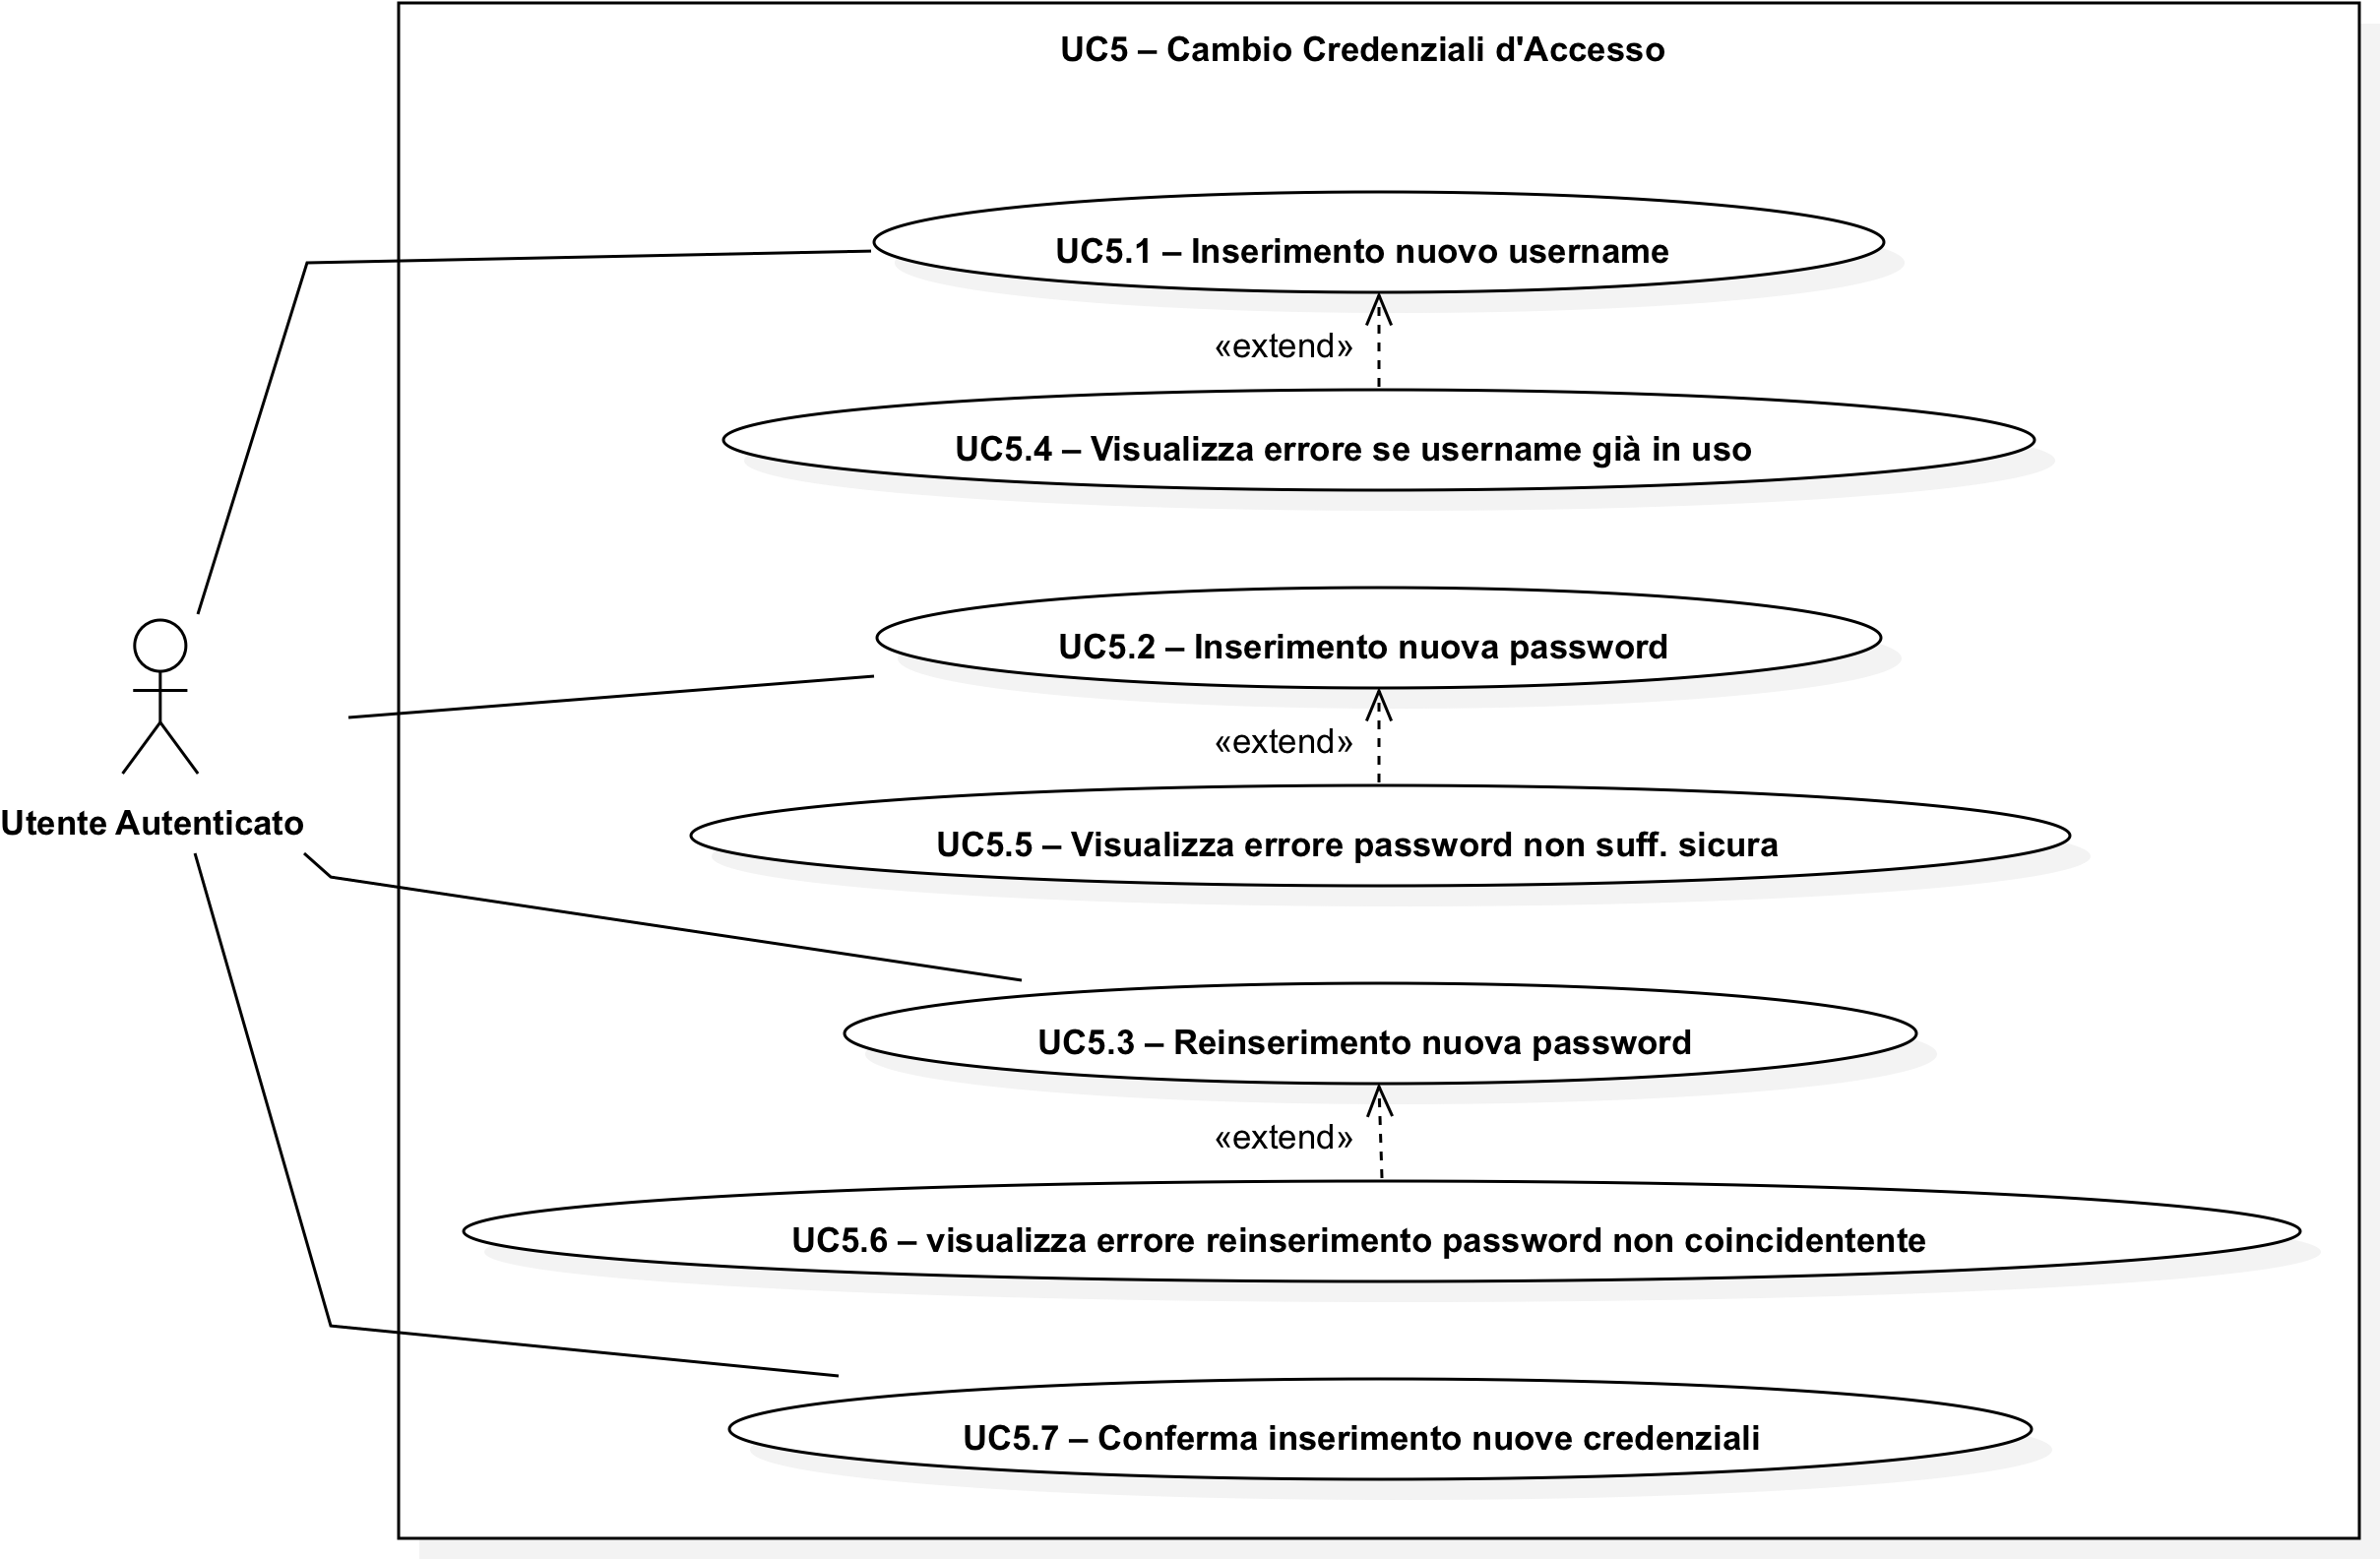
\includegraphics[scale=0.2]{img/UC5.png} 
\caption{Caso d'uso UC5 - Cambio credenziali d'accesso} 
 \end{figure} 
\desc{l'utente modifica le credenziali d'accesso.}\\\\ 
\pre{l'utente è autenticato.}\\\\ 
\post{l'utente ha modificato una o più credenziali d'accesso.}\\\\ 
\scen{\begin{itemize}
\item \UC{UC5.1} inserisci nuovo username;
\item \UC{UC5.2} inserisci nuova password;
\item \UC{UC5.3} reinserisci nuova password.
\end{itemize}}\\\\ 
\att{Utente autenticato.}

\casoduso{UC5.1}{Inserimento nuovo username} 
\desc{l'utente autenticato inserisce un nuovo username.}\\\\ 
\pre{l'utente è autenticato.}\\\\ 
\post{l'utente ha inserito un nuovo username.}\\\\ 
\scen{l'utente autenticato inserisce un nuovo username.}\\\\ 
\scensec{ESTENSIONE \begin{itemize}
\item \UC{UC5.4} l'username inserito è già in uso e viene visualizzato l'errore.
\end{itemize}}\\\\ 
\att{Utente autenticato.}

\casoduso{UC5.2}{Inserimento nuova password} 
\desc{l'utente autenticato inserisce una nuova password.}\\\\ 
\pre{l'utente è autenticato.}\\\\ 
\post{l'utente ha inserito una nuova password.}\\\\ 
\scen{l'utente autenticato inserisce una nuova password.}\\\\ 
\scensec{ESTENSIONE \begin{itemize}
\item \UC{UC5.5}la password inserita non è sufficientemente sicura e viene visualizzato l'errore.
\end{itemize}}\\\\ 
\att{Utente autenticato.}

\casoduso{UC5.3}{Reinserimento nuova password} 
\desc{l'utente autenticato reinserisce la nuova password.}\\\\ 
\pre{l'utente è autenticato.}\\\\ 
\post{l'utente ha reinserito la nuova password.}\\\\ 
\scen{l'utente autenticato reinserisce la nuova password.}\\\\ 
\scensec{ESTENSIONE \begin{itemize}
\item \UC{UC5.6}la password reinserita non coincide con la nuova password e viene visualizzato l'errore.
\end{itemize}}\\\\ 
\att{Utente autenticato.}

\casoduso{UC5.4}{Visualizza errore username già in uso} 
\desc{l'utente visualizza l'errore il quale segnala che l'username inserito è già in uso.}\\\\ 
\pre{l'utente ha inserito un nuovo username già in uso.}\\\\ 
\post{l'utente ha visualizzato il messaggio di errore di username già in uso.}\\\\ 
\scen{l'utente visualizza l'errore il quale segnala che l'username inserito è già in uso.}\\\\ 
\att{Utente autenticato.}

\casoduso{UC5.5}{Visualizza errore password non sufficientemente sicura} 
\desc{l'utente visualizza l'errore il quale segnala che la nuova password inserita non è sufficientemente sicura.}\\\\ 
\pre{l'utente ha inserito una nuova password non sufficientemente sicura.}\\\\ 
\post{l'utente ha visualizzato l'errore il quale segnala che la nuova password inserita non è sufficientemente sicura.}\\\\ 
\scen{l'utente visualizza l'errore il quale segnala che la nuova password inserita non è sufficientemente sicura.}\\\\ 
\att{Utente autenticato.}

\casoduso{UC5.6}{Visualizza errore password reinserita non coincidente con la nuova password} 
\desc{l'utente visualizza l'errore il quale segnala che la password reinserita non coincide con la nuova password.}\\\\ 
\pre{l'utente ha reinserito la password che non coincide con quella nuova precedentemente inserita.}\\\\ 
\post{l'utente ha visualizzato l'errore il quale segnala che la password reinserita non coincide con la nuova password.}\\\\ 
\scen{l'utente visualizza l'errore il quale segnala che la password reinserita non coincide con la nuova password.}\\\\ 
\att{Utente autenticato.}

\casoduso{UC5.7}{Conferma inserimento nuove credenziali} 
\desc{l'utente autenticato conferma l'inserimento delle nuove credenziali.}\\\\ 
\pre{l'utente ha inserito le credenziali da modificare.}\\\\ 
\post{l'utente ha confermato l'inserimento delle nuove credenziali.}\\\\ 
\scen{l'utente autenticato conferma l'inserimento delle nuove credenziali.}\\\\ 
\att{Utente autenticato.}

\casoduso{UC6}{Cerca edifici} 
\desc{l'utente cerca edifici abilitati.}\\\\ 
\pre{l'utente ha l'app installata e in esecuzione.}\\\\ 
\post{l'utente ha visualizzato gli edifici abilitati.}\\\\ 
\scen{l'utente cerca edifici abilitati.}\\\\ 
\scensec{ESTENSIONE:
\begin{itemize}
\item \UC{UC12} il GPS non è attivo e viene visualizzato l'invito ad attivarlo;
\item \UC{UC13} la connessione ad internet non è attiva e viene visualizzato l'invito ad attivarla.
\end{itemize}}\\\\ 
\att{Utente.}

\casoduso{UC7}{Cerca edifici per raggio} 
\begin{figure}[H] 
\centering 
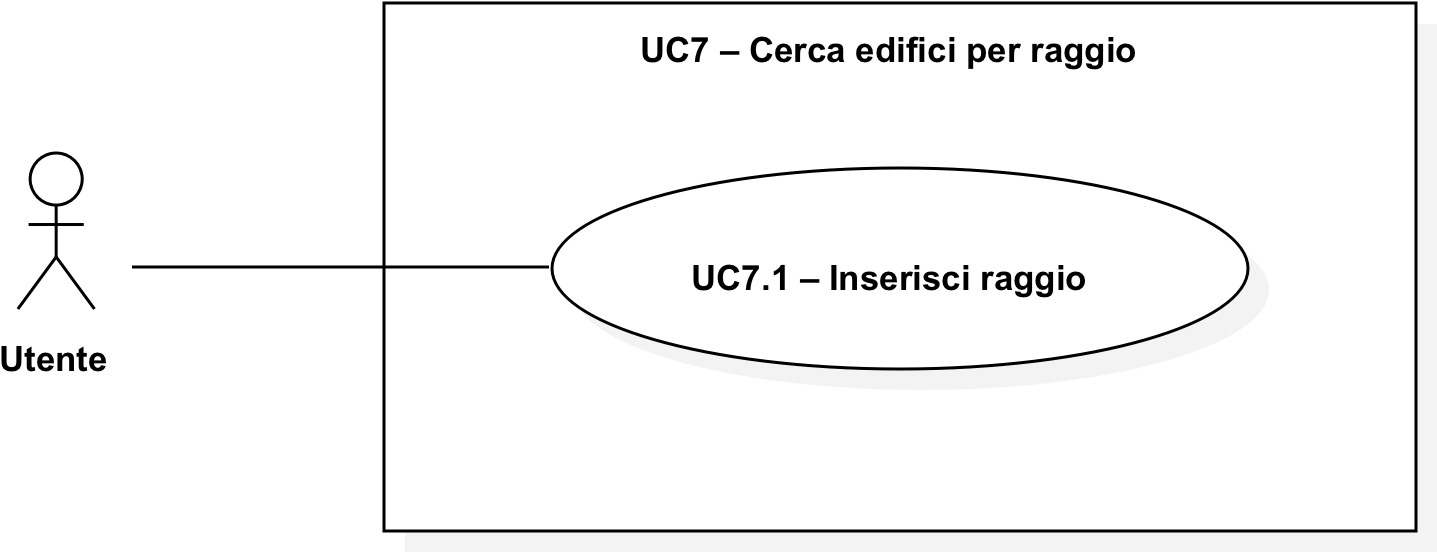
\includegraphics[scale=0.2]{img/UC7.png} 
\caption{Caso d'uso UC7 - Cerca edifici per raggio} 
 \end{figure} 
\desc{l'utente cerca gli edifici abilitati entro un raggio.}\\\\ 
\pre{l'utente è alla ricerca degli edifici abilitati.}\\\\ 
\post{l'utente ha cercato gli edifici abilitati.}\\\\ 
\scen{l'utente cerca gli edifici abilitati entro un raggio tramite \UC{UC7.1}.
}\\\\ 
\att{Utente.}

\casoduso{UC7.1}{Inserisci raggio} 
\desc{l'utente inserisce il raggio di ricerca degli edifici abilitati.}\\\\ 
\pre{l'utente è alla ricerca degli edifici abilitati.}\\\\ 
\post{l'utente ha inserito il raggio di ricerca degli edifici abilitati.}\\\\ 
\scen{l'utente inserisce il raggio di ricerca degli edifici abilitati.}\\\\ 
\att{Utente.}

\casoduso{UC9}{Visualizza lista edifici} 
\desc{l'utente visualizza la lista degli edifici abilitati.}\\\\ 
\pre{l'utente ha cercato gli edifici.}\\\\ 
\post{l'utente ha visualizzato la lista degli edifici.}\\\\ 
\scen{l'utente visualizza la lista degli edifici abilitati.}\\\\ 
\att{Utente.}

